\documentclass [11pt, letterpaper] {article}
\input {headings}
\newcommand \recipeName {Spaetzle}
\newcommand \fileName {Spaetzle}
\chead {\recipeName}

\begin {document}
\input {title}

\begin {flushright}
{Adapted from {\it Lidia's Italian Table} by Lidia Bastianich and from Canteen's chef Mike Nguyen's recipe in {\it Edmonton Cooks} }
\end {flushright}

This recipe uses almond milk and later cooks the Spaetzle in olive oil to avoid milk products. If you can use milk products, you should use whole milk and later cook the Spaetzle in butter.

\vspace{0.3in}
\begin{description}

\item[Ingredients:]\ \\
	\begin{itemize}
	\item 1/2 cup of cornmeal (2 oz = 60 grams)
	\item 1 cup of boiling water (8 oz = 240 grams)2 
	\item 2 cups of almond milk (18 oz) (or regular milk)
	\item 8 eggs
	\item 1 tablespoon + 1 teaspoon of salt
	\item 1 teaspoon of freshly ground black pepper
	\item 1/2 teaspoon of freshly grated nutmeg
	\item	5 cups of all-purpose flour (more as needed)
	\item Olive oil (or a combination of canola oil and butter)
	\end{itemize}

\item[Procedure:]\ \\
	\begin{description}
	\item[Bloom the cornmeal]\ \\
		\begin{itemize}
			\item	Put cornmeal at the bottom of a large standing mixer bowl (you may also put in a regular large bowl if you will  mix by hand with a balloon whisk)   
			\item Pour the fast boiling water over the corn meal and briefly stir to ensure that there are no lumps.
			\item Let stand, uncovered, for at least 10 minutes.
		\end{itemize}
	\item[Prepare the batter]\ \\
		\begin{itemize}
			\item Slowly add about half a cup of the almond milk to the corn mush mixing with a balloon whisk to ensure that there are no lumps.
			\item Break the eggs over the mixture and mix with the whisk until incorporated.
			\item Add the remainder of almond milk, salt, black pepper and nutmeg and stir until homogeneous.
			\item Put the dough hook in the mixer and turn it to medium speed. 
			\item Slowly add the flour so that it gets well mixed into the batter without forming large lumps.
			\item The batter should be fairly thick but still pourable. Add more flour if it is too thin. Or more milk if it is becoming too thick. It is difficult to thin the batter if it gets too thick, thus watch how much flour you add.
			\item Once the batter is at the right consistence, beat it with the mixer in moderately high speed for 3 to 5 minutes scraping the sides of the bowl every minute or so to ensure that the batter is well mixed.
			\item (If mixing by hand, you can switch to a wooden spoon and beat the batter for several minutes).
			\item Let the batter rest for at least 30 minutes. It can stand like this at room temperature for several hours. Best to not refrigerate. But if you do, take it out a few hours before cooking so that it can be at room temperature.
		\end{itemize}
	\item[Cook the Spaetzle]\ \\
		\begin{itemize}
			\item Bring a large pot of water to a boil and add 1-2 tablespoon (water should taste slightly salted). 
			\item Oil a large rimmed baking sheet with plenty of olive oil (use canola oil for the regular milk version that you will cook in butter).
			\item Place a pasta colander over a large bowl.
			\item Dunk your spaetzle maker into the hot water. 
			\item Fill the container with the batter and cut the spaetzle by moving the container back and forth over the boiling water.
			\item Using a mesh strainer, gently lift the spaetzle from the bottom of the pan once to ensure that it will not stick to the bottom.
			\item A couple of minutes after the spaetzle floats, collect the spaetzle from the boiling water and place in the colander over the bowl.
			\item Let is stand in the colander for a few minutes for most of the water to drain.
			\item Transfer spaetzle to the oiled baking sheet and stir, add a bit more olive (or canola) oil if needed.
			\item Repeat the cooking process until all the batter is used up --- this is a large recipe, if the water becomes too thick with flour from the spaetzle, you may have to start with a fresh pot of water.
			\item Let the spaetzle cool completely, turning it over from time to time.
			\item It is best if the spaetzle sits in the baking sheet for several hours at room temperature so that it dry some.
			\item You can put it in plastic containers and refrigerate or freeze at this point.
		\end{itemize}
	\item[Browning the Spaetzle]\ \\
		\begin{itemize}
			\item In a non-stick pan, warm up a few tablespoons of olive oil (you can use butter if not concerned with dairy products). 
			\item Put the portion of spaetzle that you want to serve in the hot oil (or butter) let it seat for a couple of minutes and then start stir frying it but stir gently to keep the spaetzle intact.
			\item Cook, stirring until the spaetzle is completely warmed up and there are a few brown spots in some of them.
			\item Sprinkle with freshly black pepper.
			\item Serve with a sauce or simply sprinkled with parmesan cheese.
		\end{itemize}
	\end{description}
\end{description}

\begin{table}
\begin{tabular}{cccc}
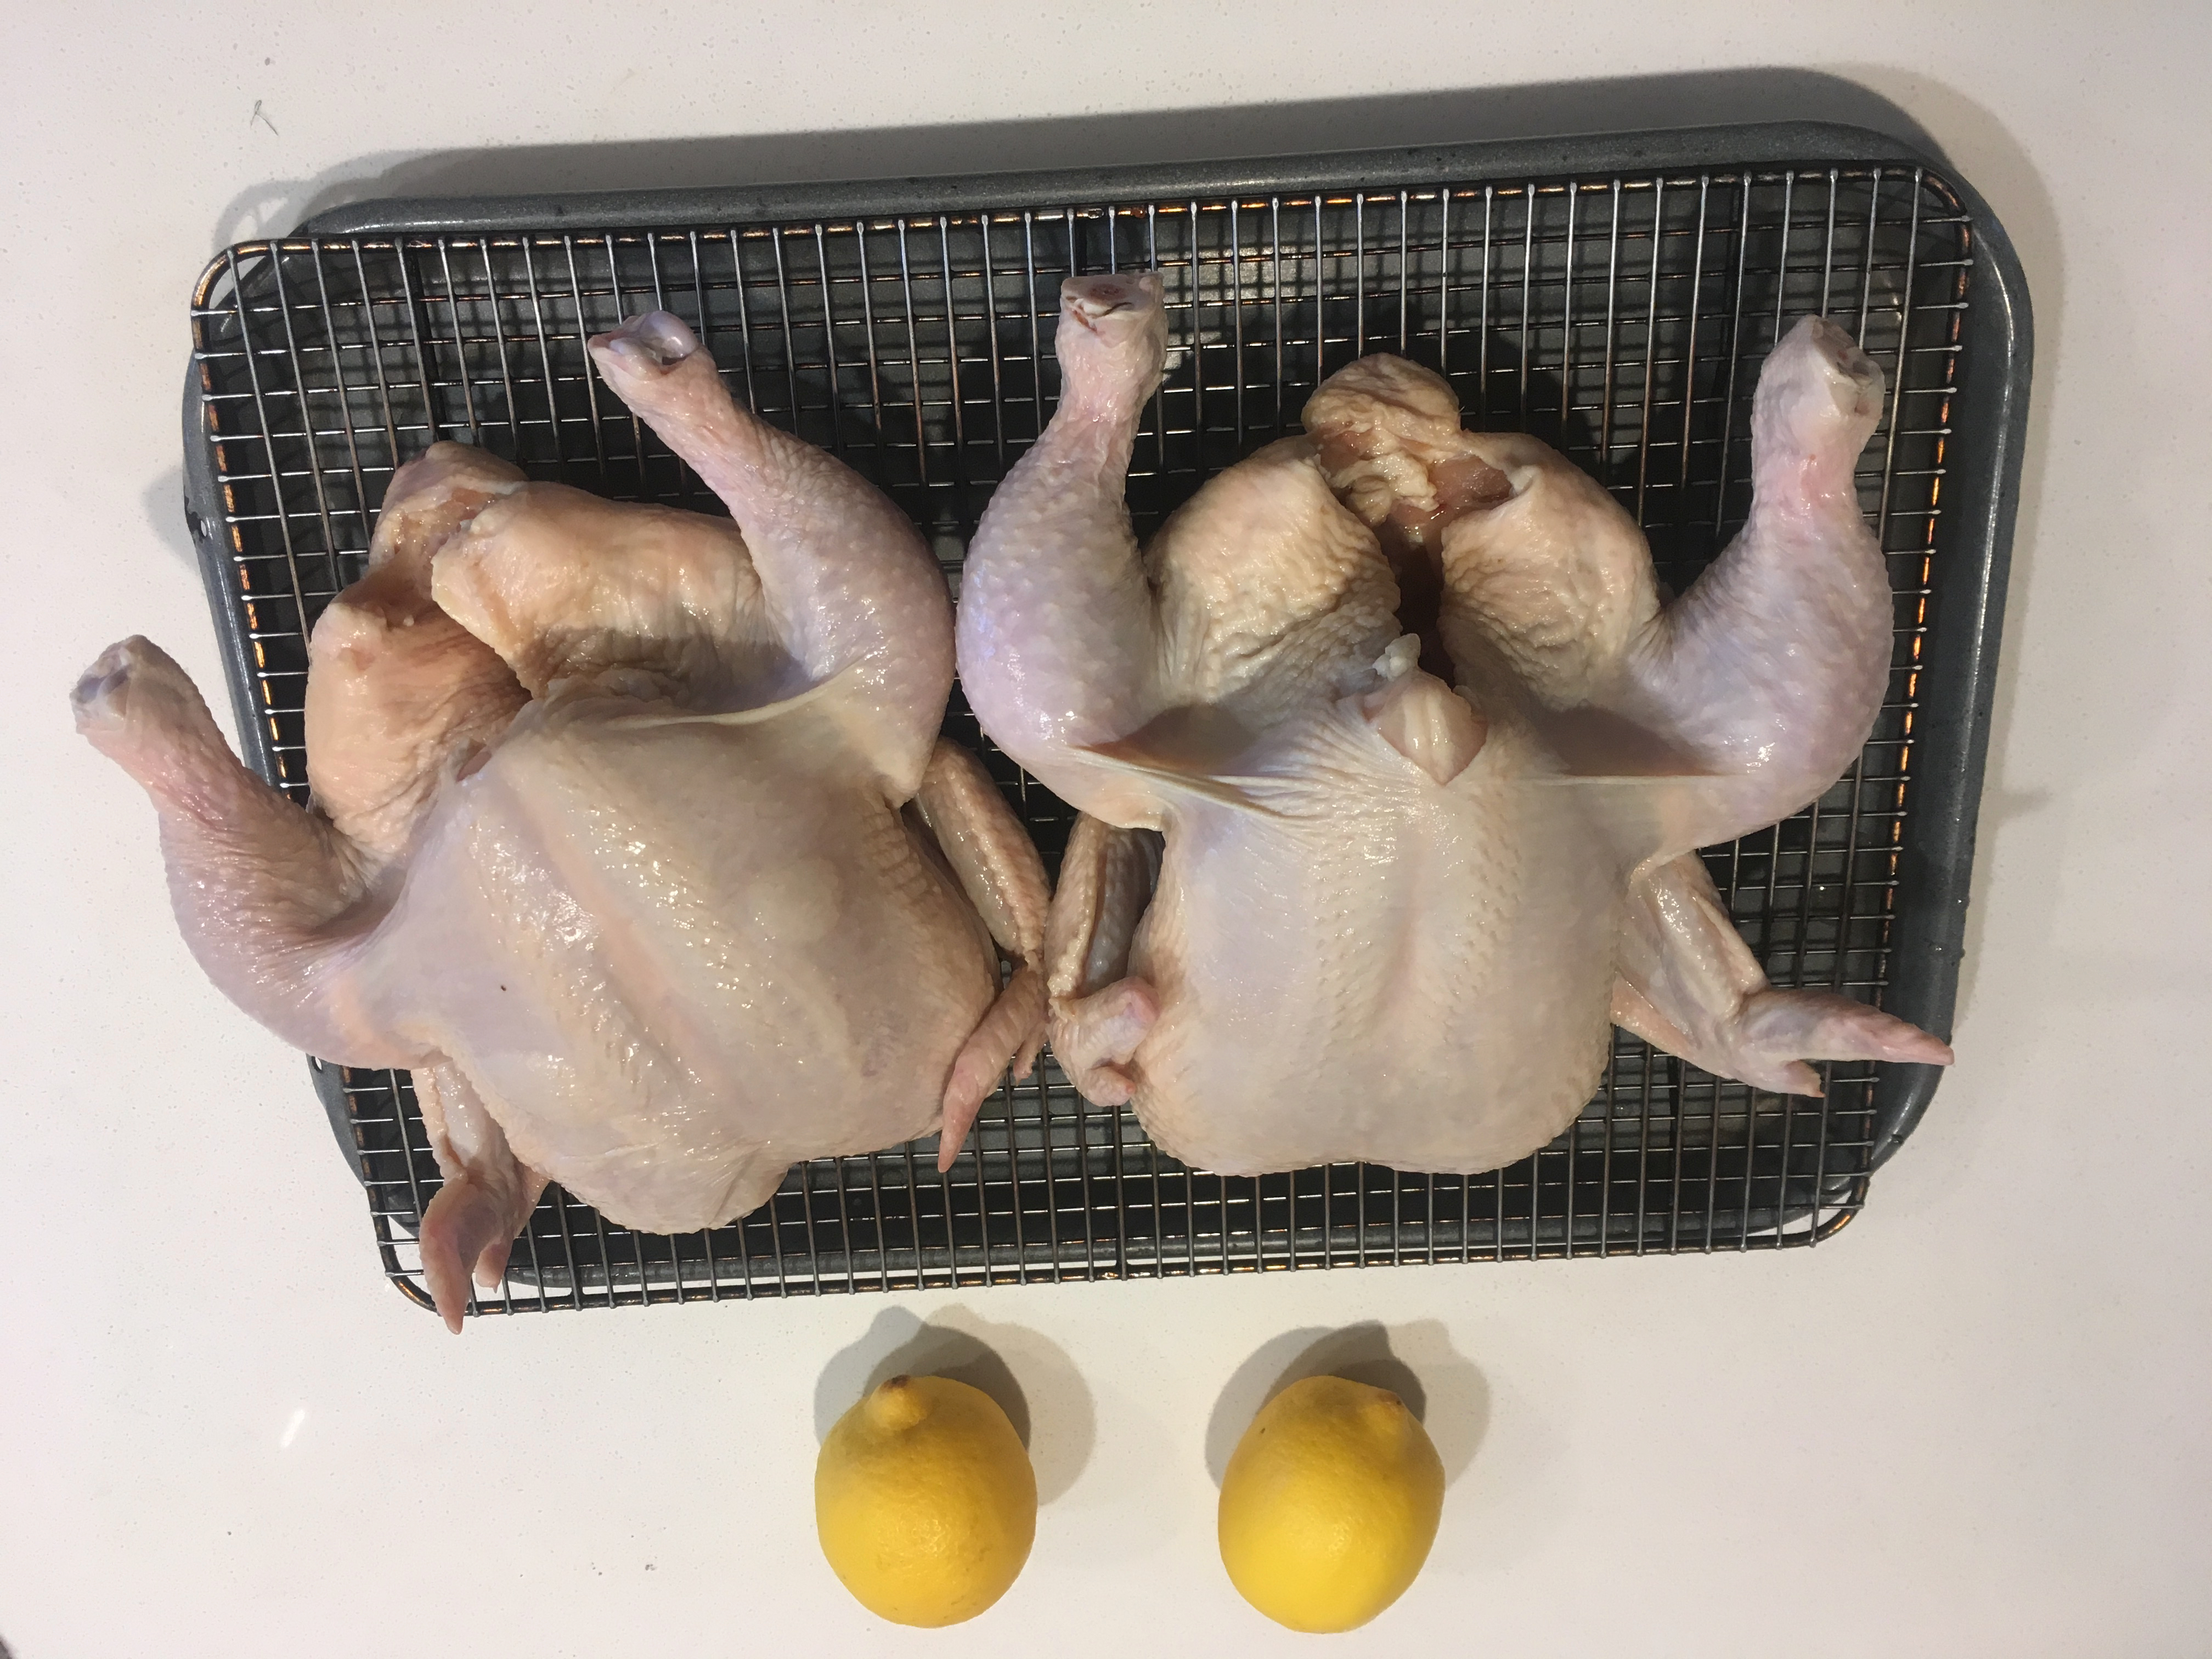
\includegraphics[width=0.25\textwidth]{\imageDir/\fileName/IMG_3197.jpg} &
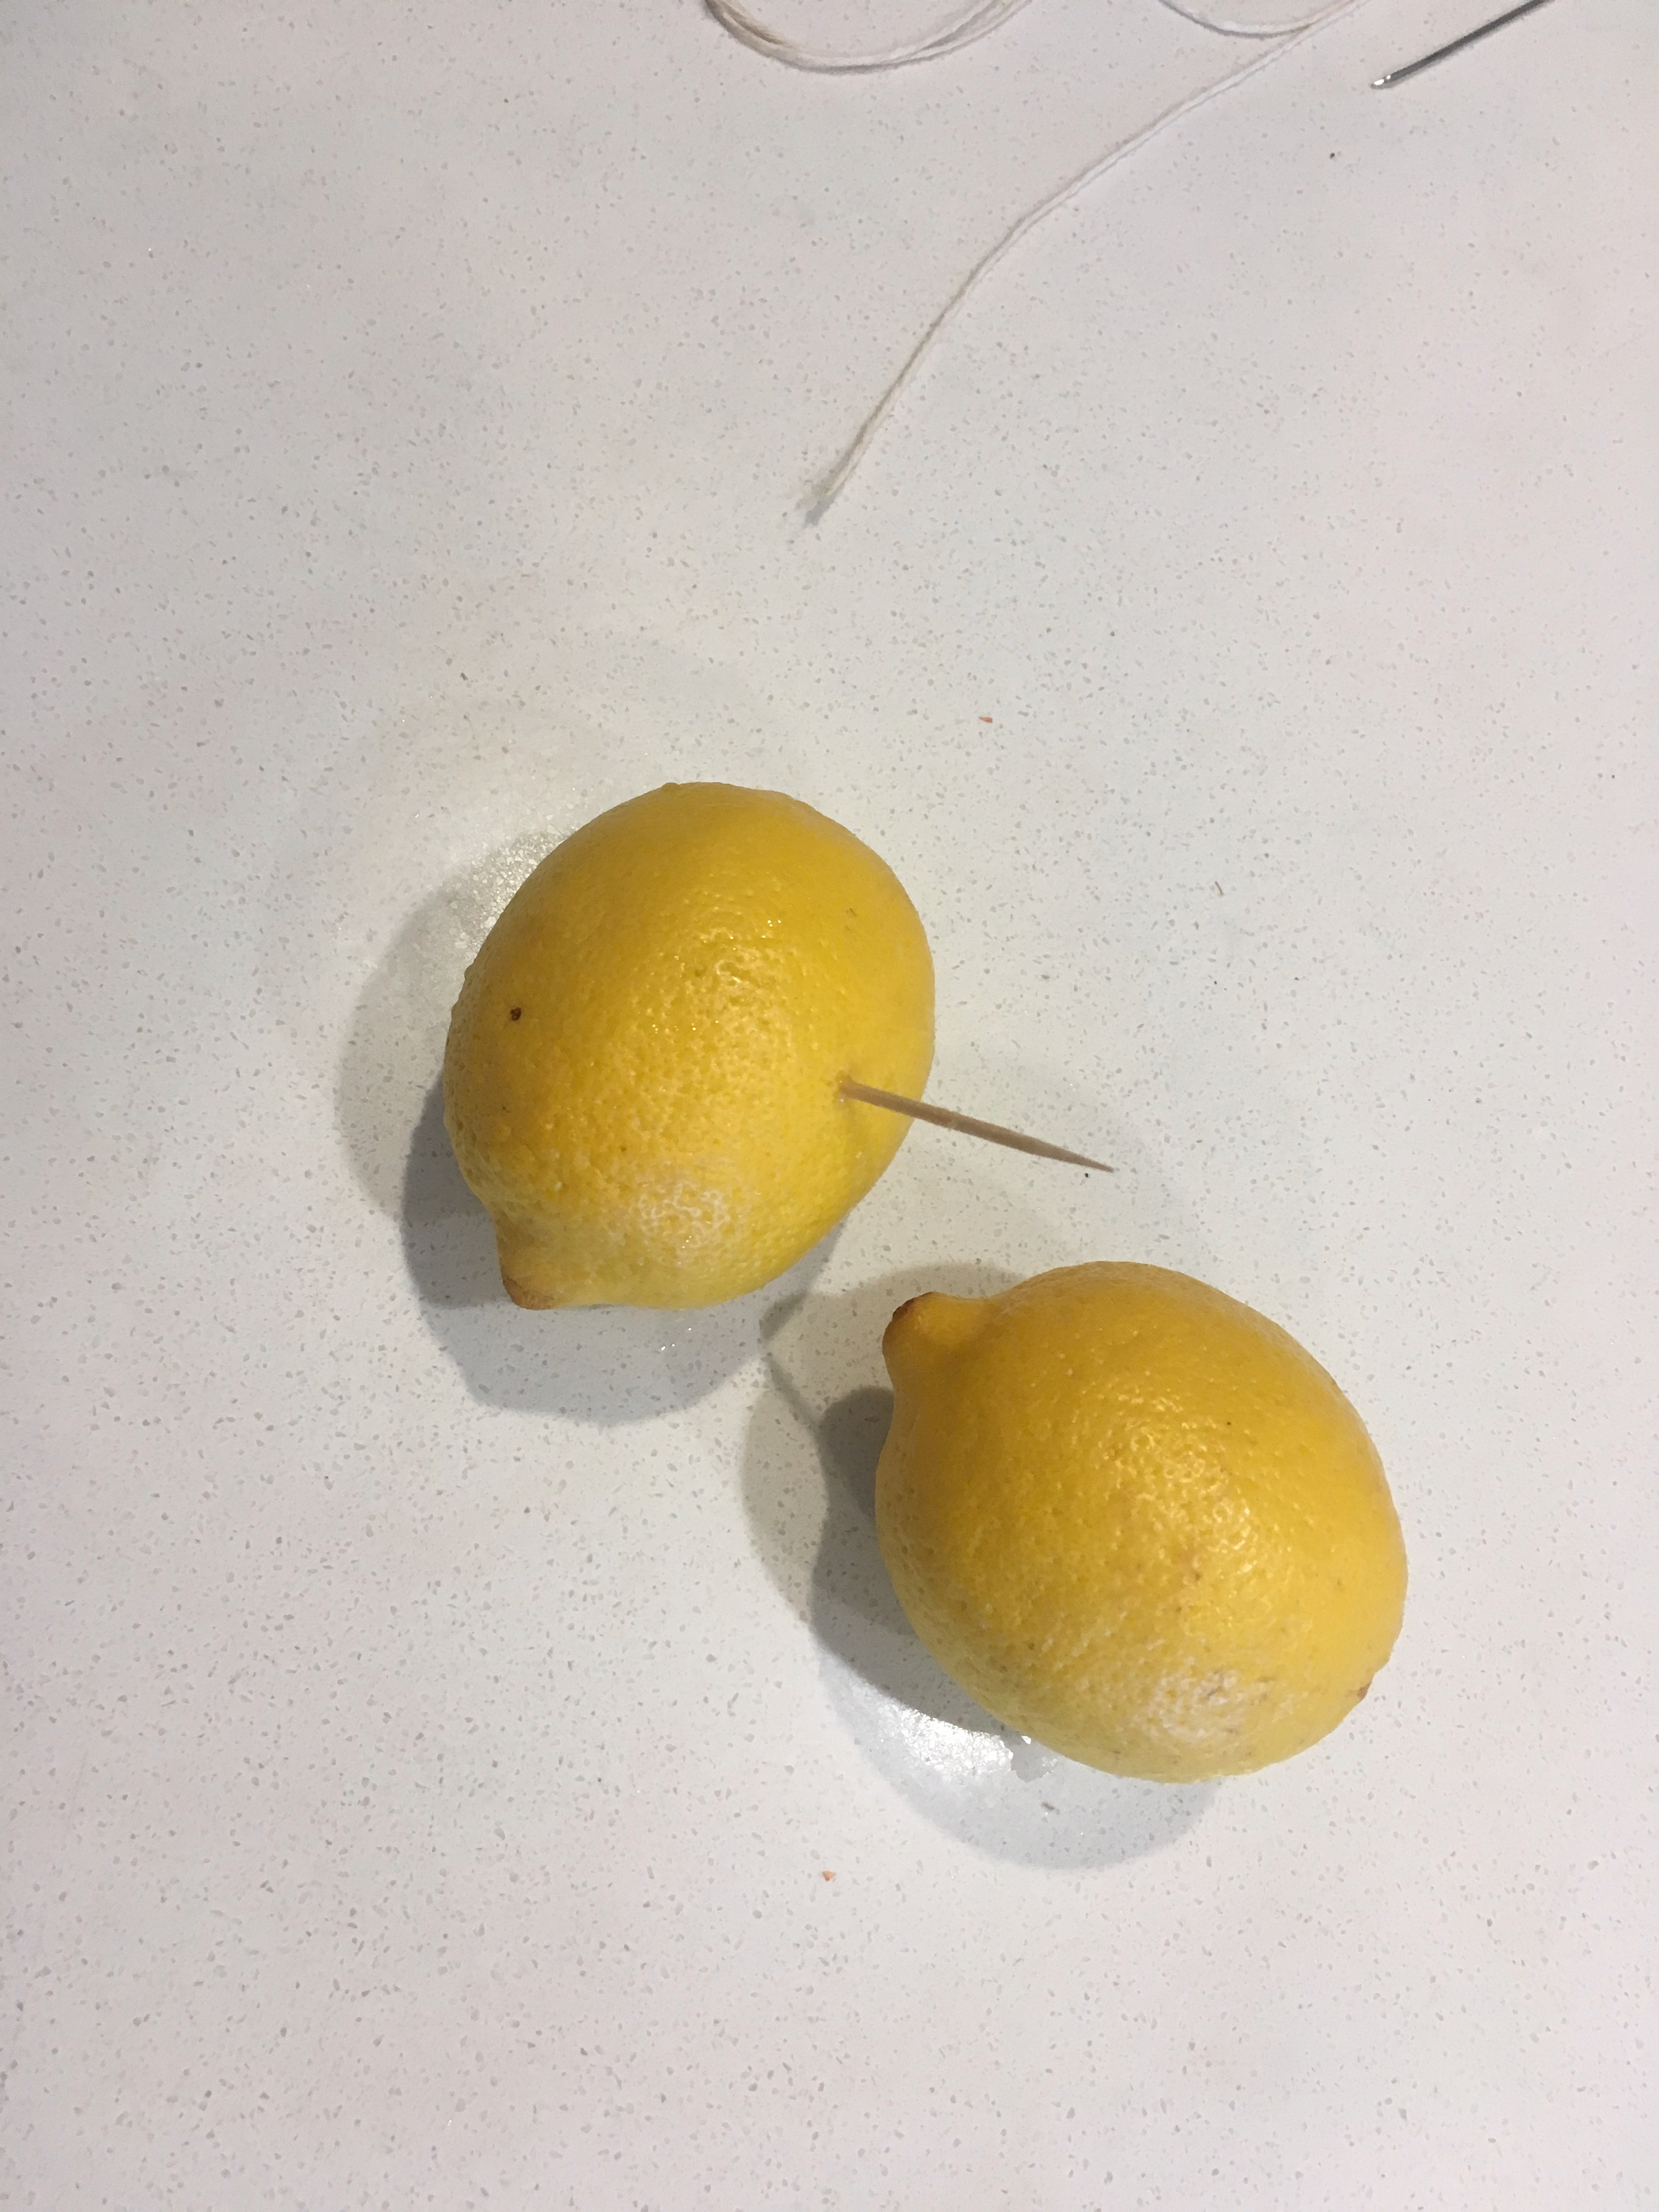
\includegraphics[width=0.25\textwidth]{\imageDir/\fileName/IMG_3212.jpg} &
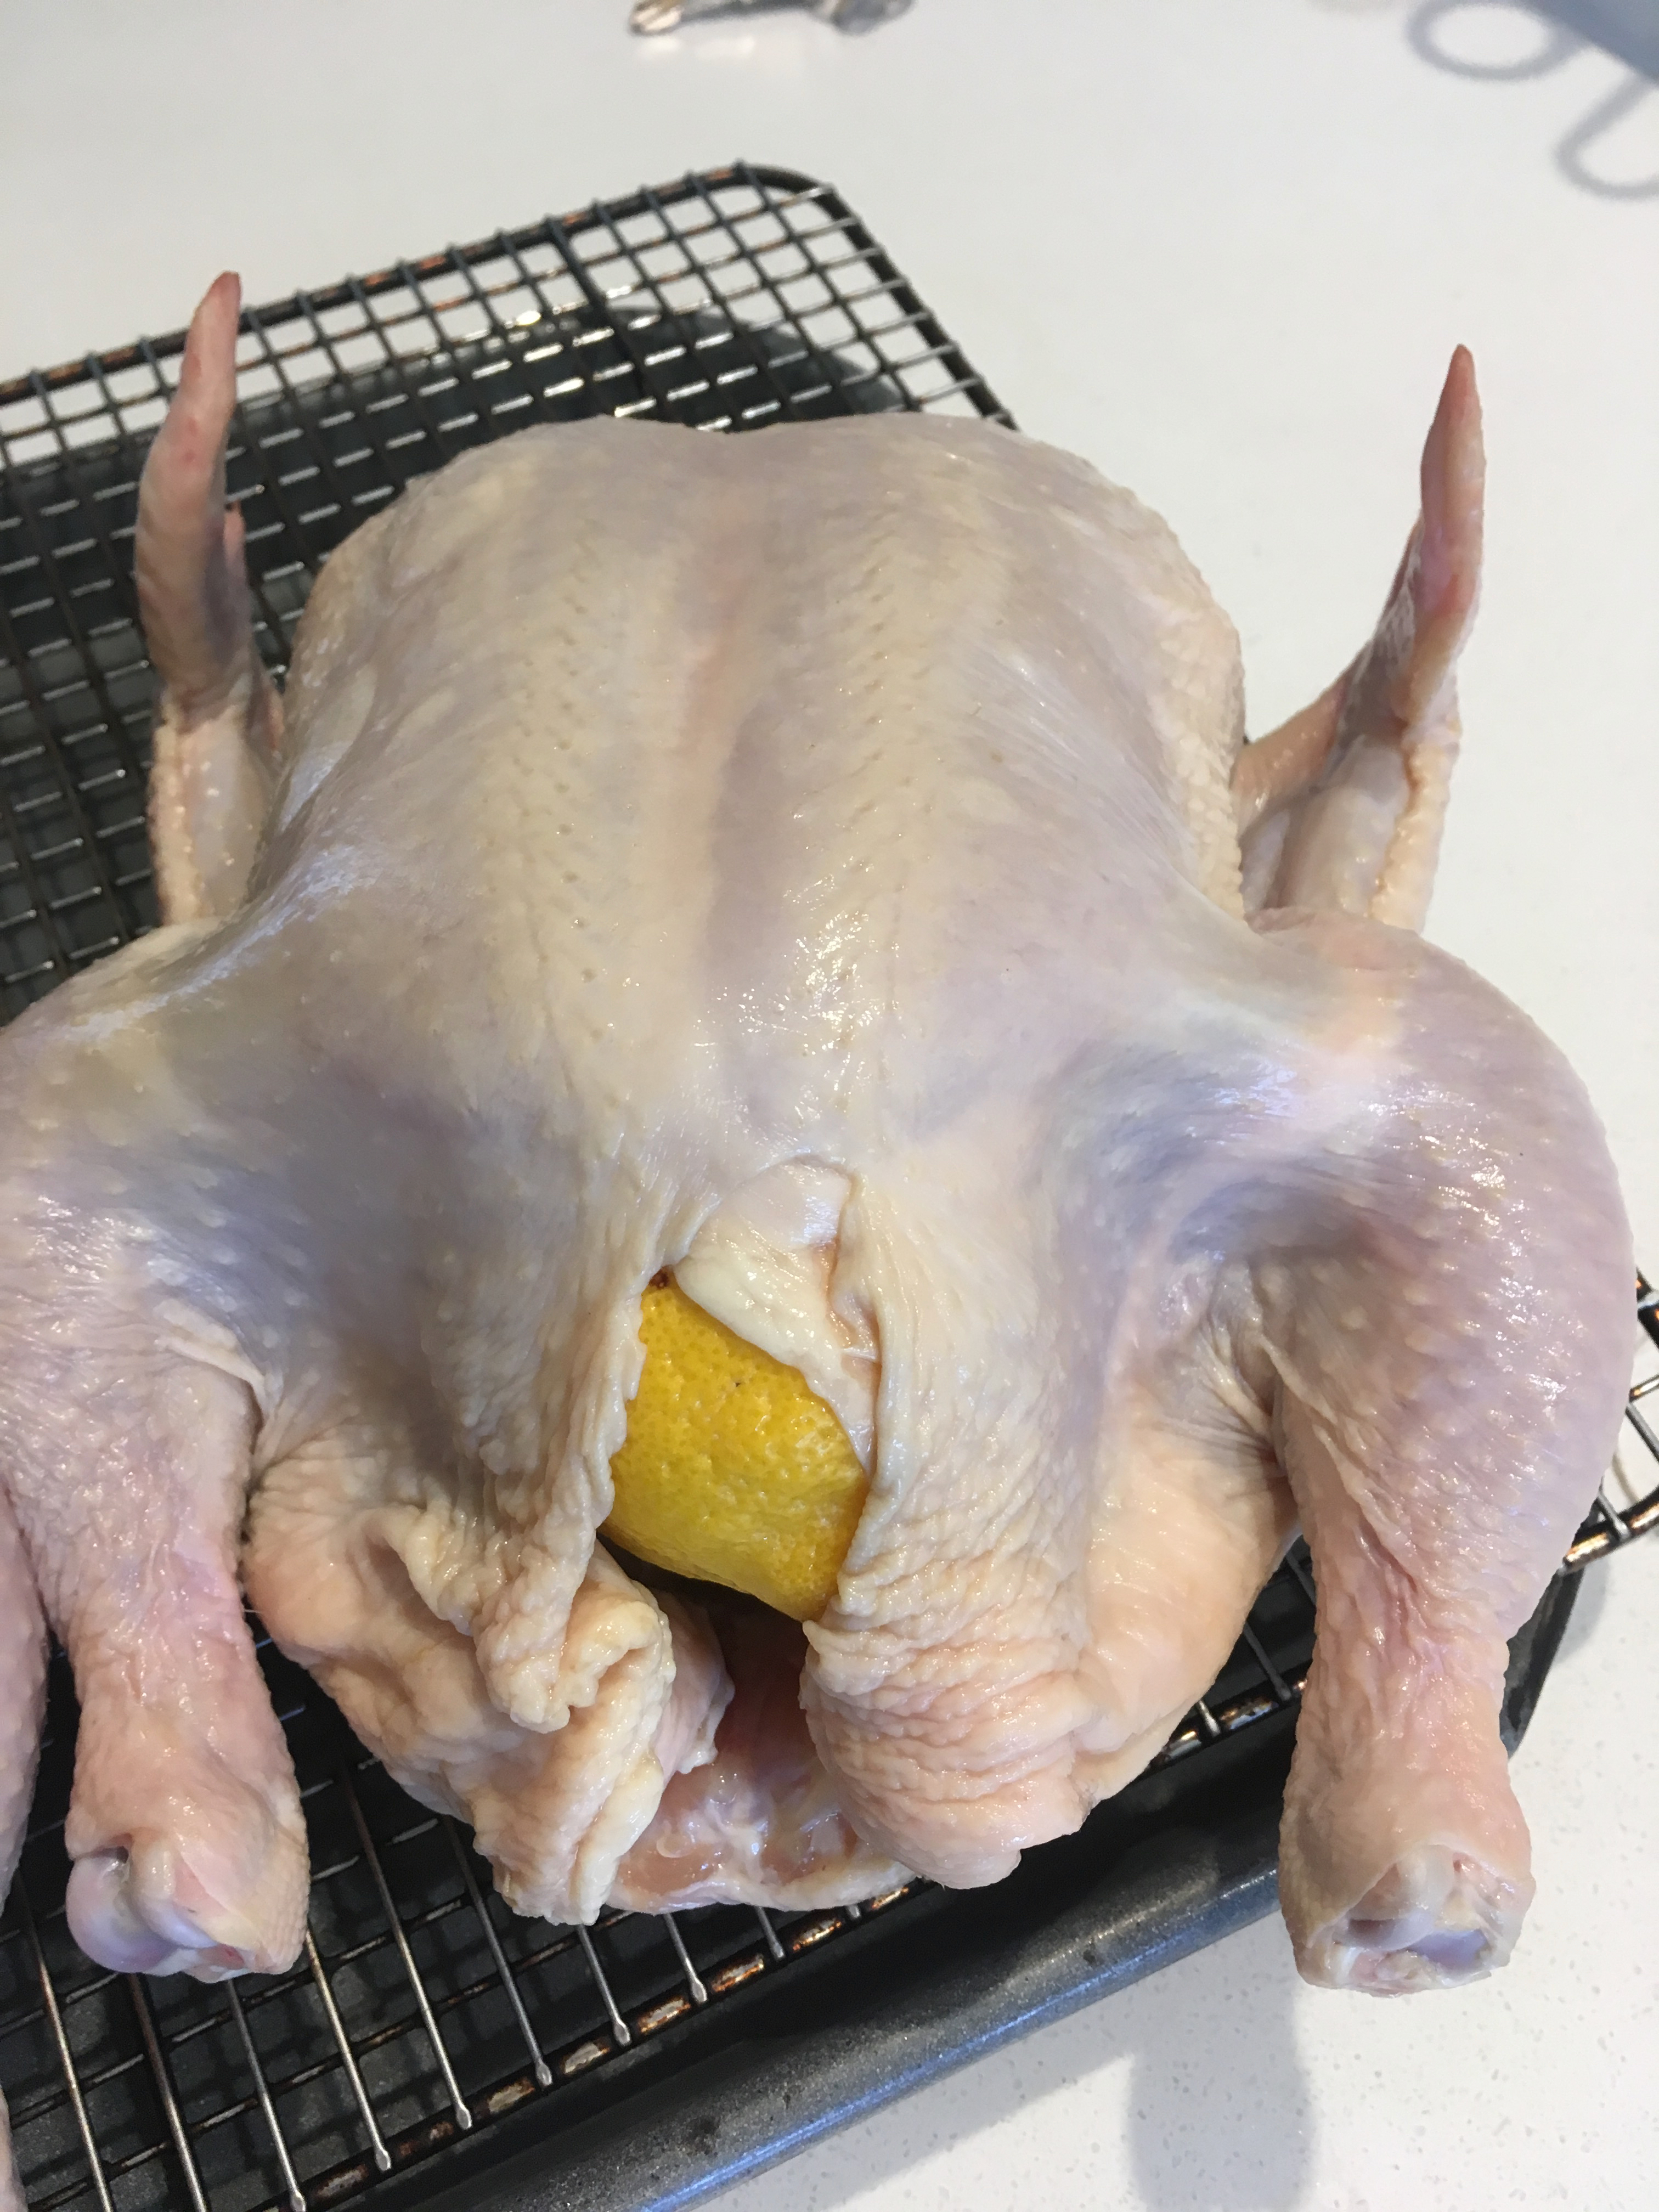
\includegraphics[width=0.25\textwidth]{\imageDir/\fileName/IMG_3213.jpg} \\
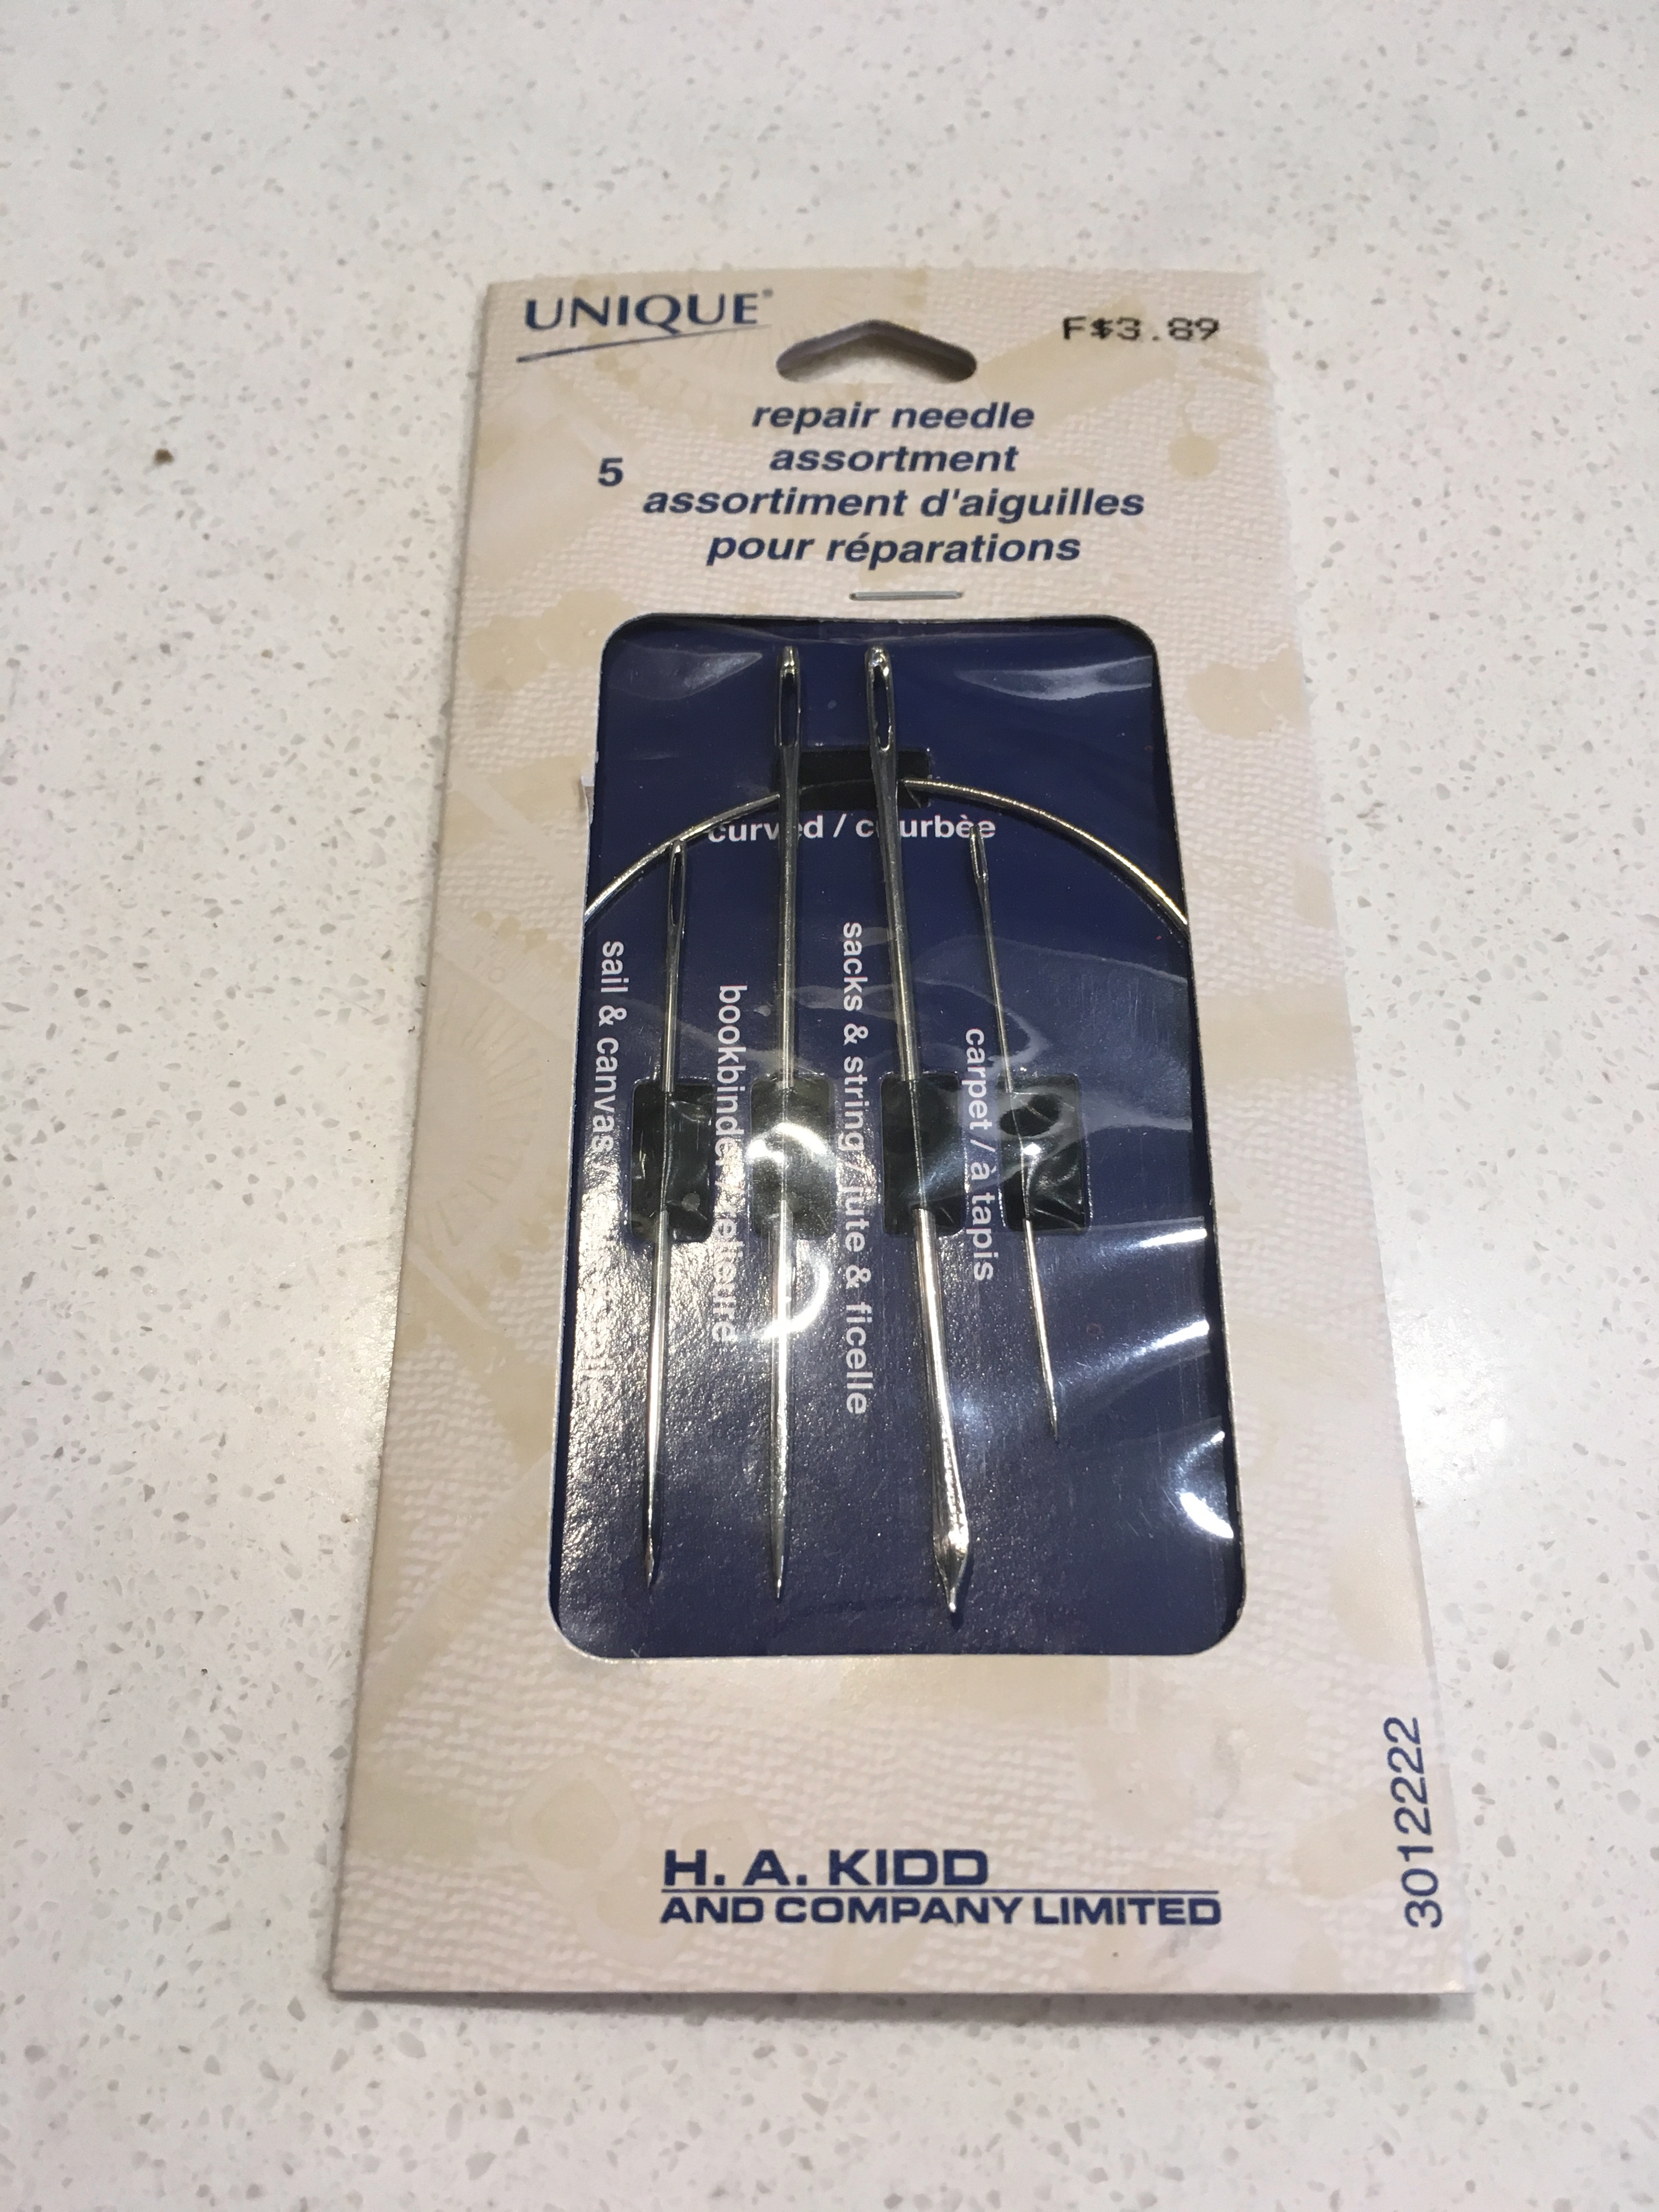
\includegraphics[width=0.25\textwidth]{\imageDir/\fileName/IMG_3206.jpg} &
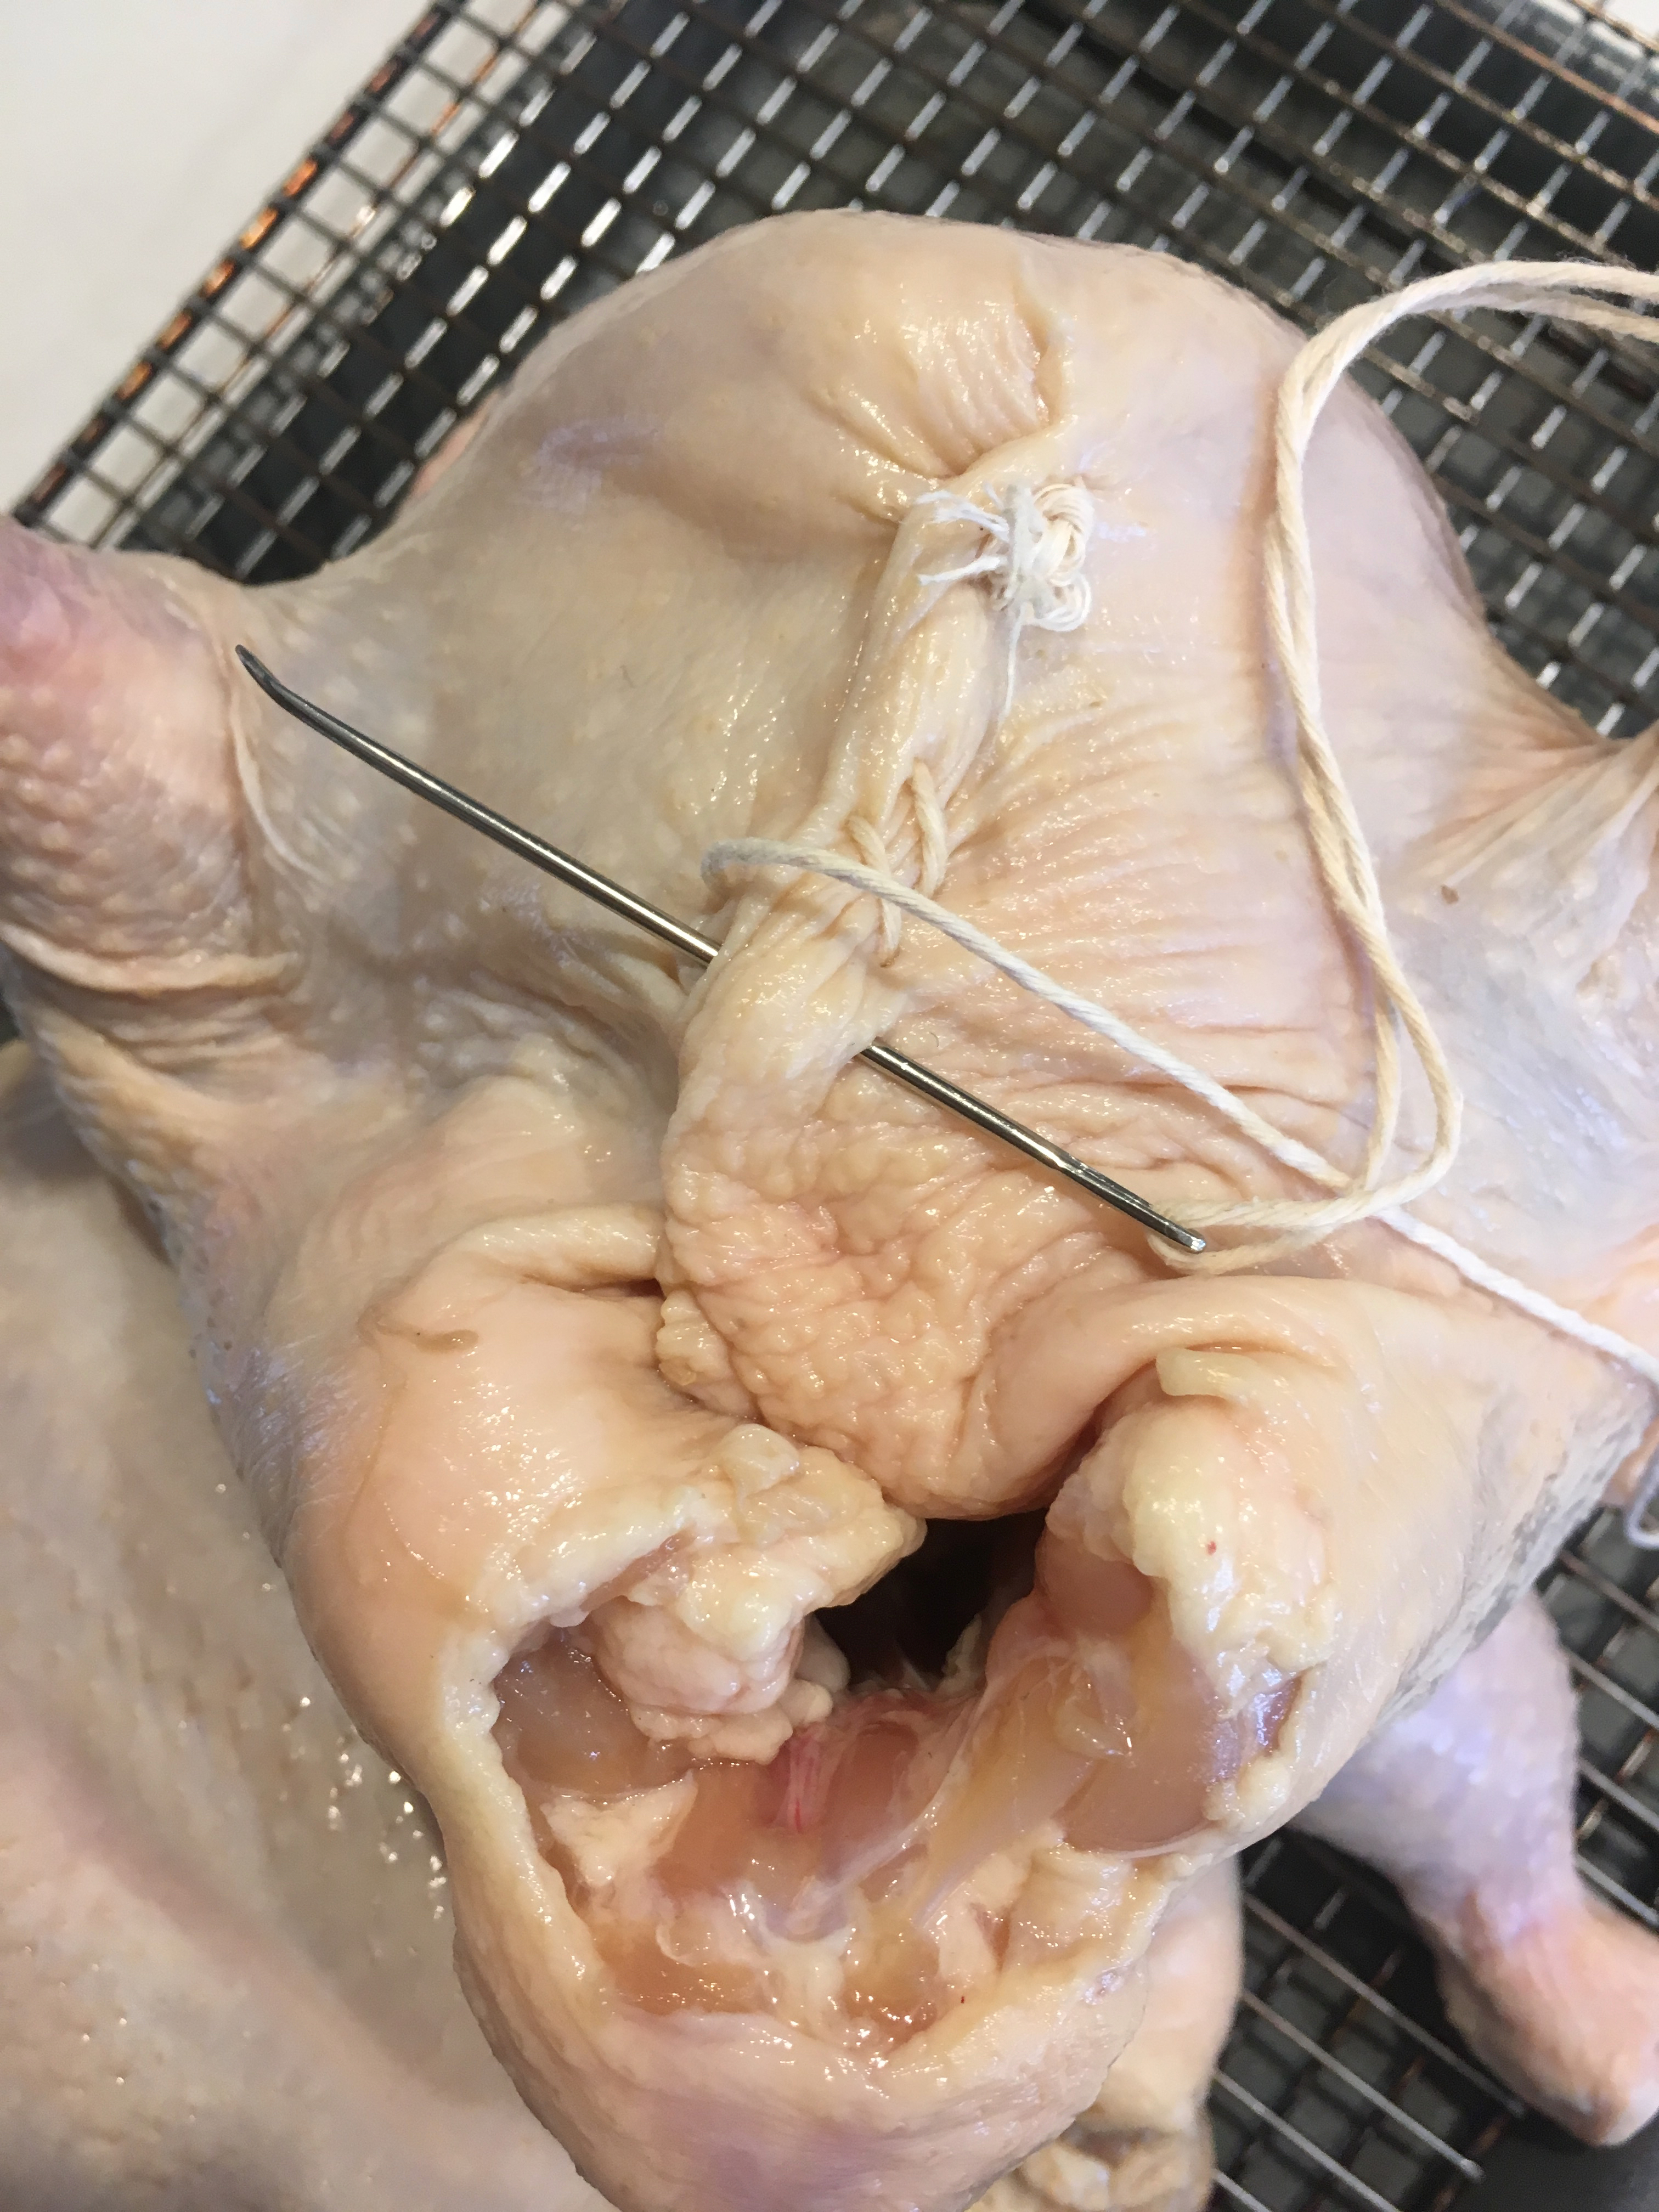
\includegraphics[width=0.25\textwidth]{\imageDir/\fileName/IMG_3214.jpg} &
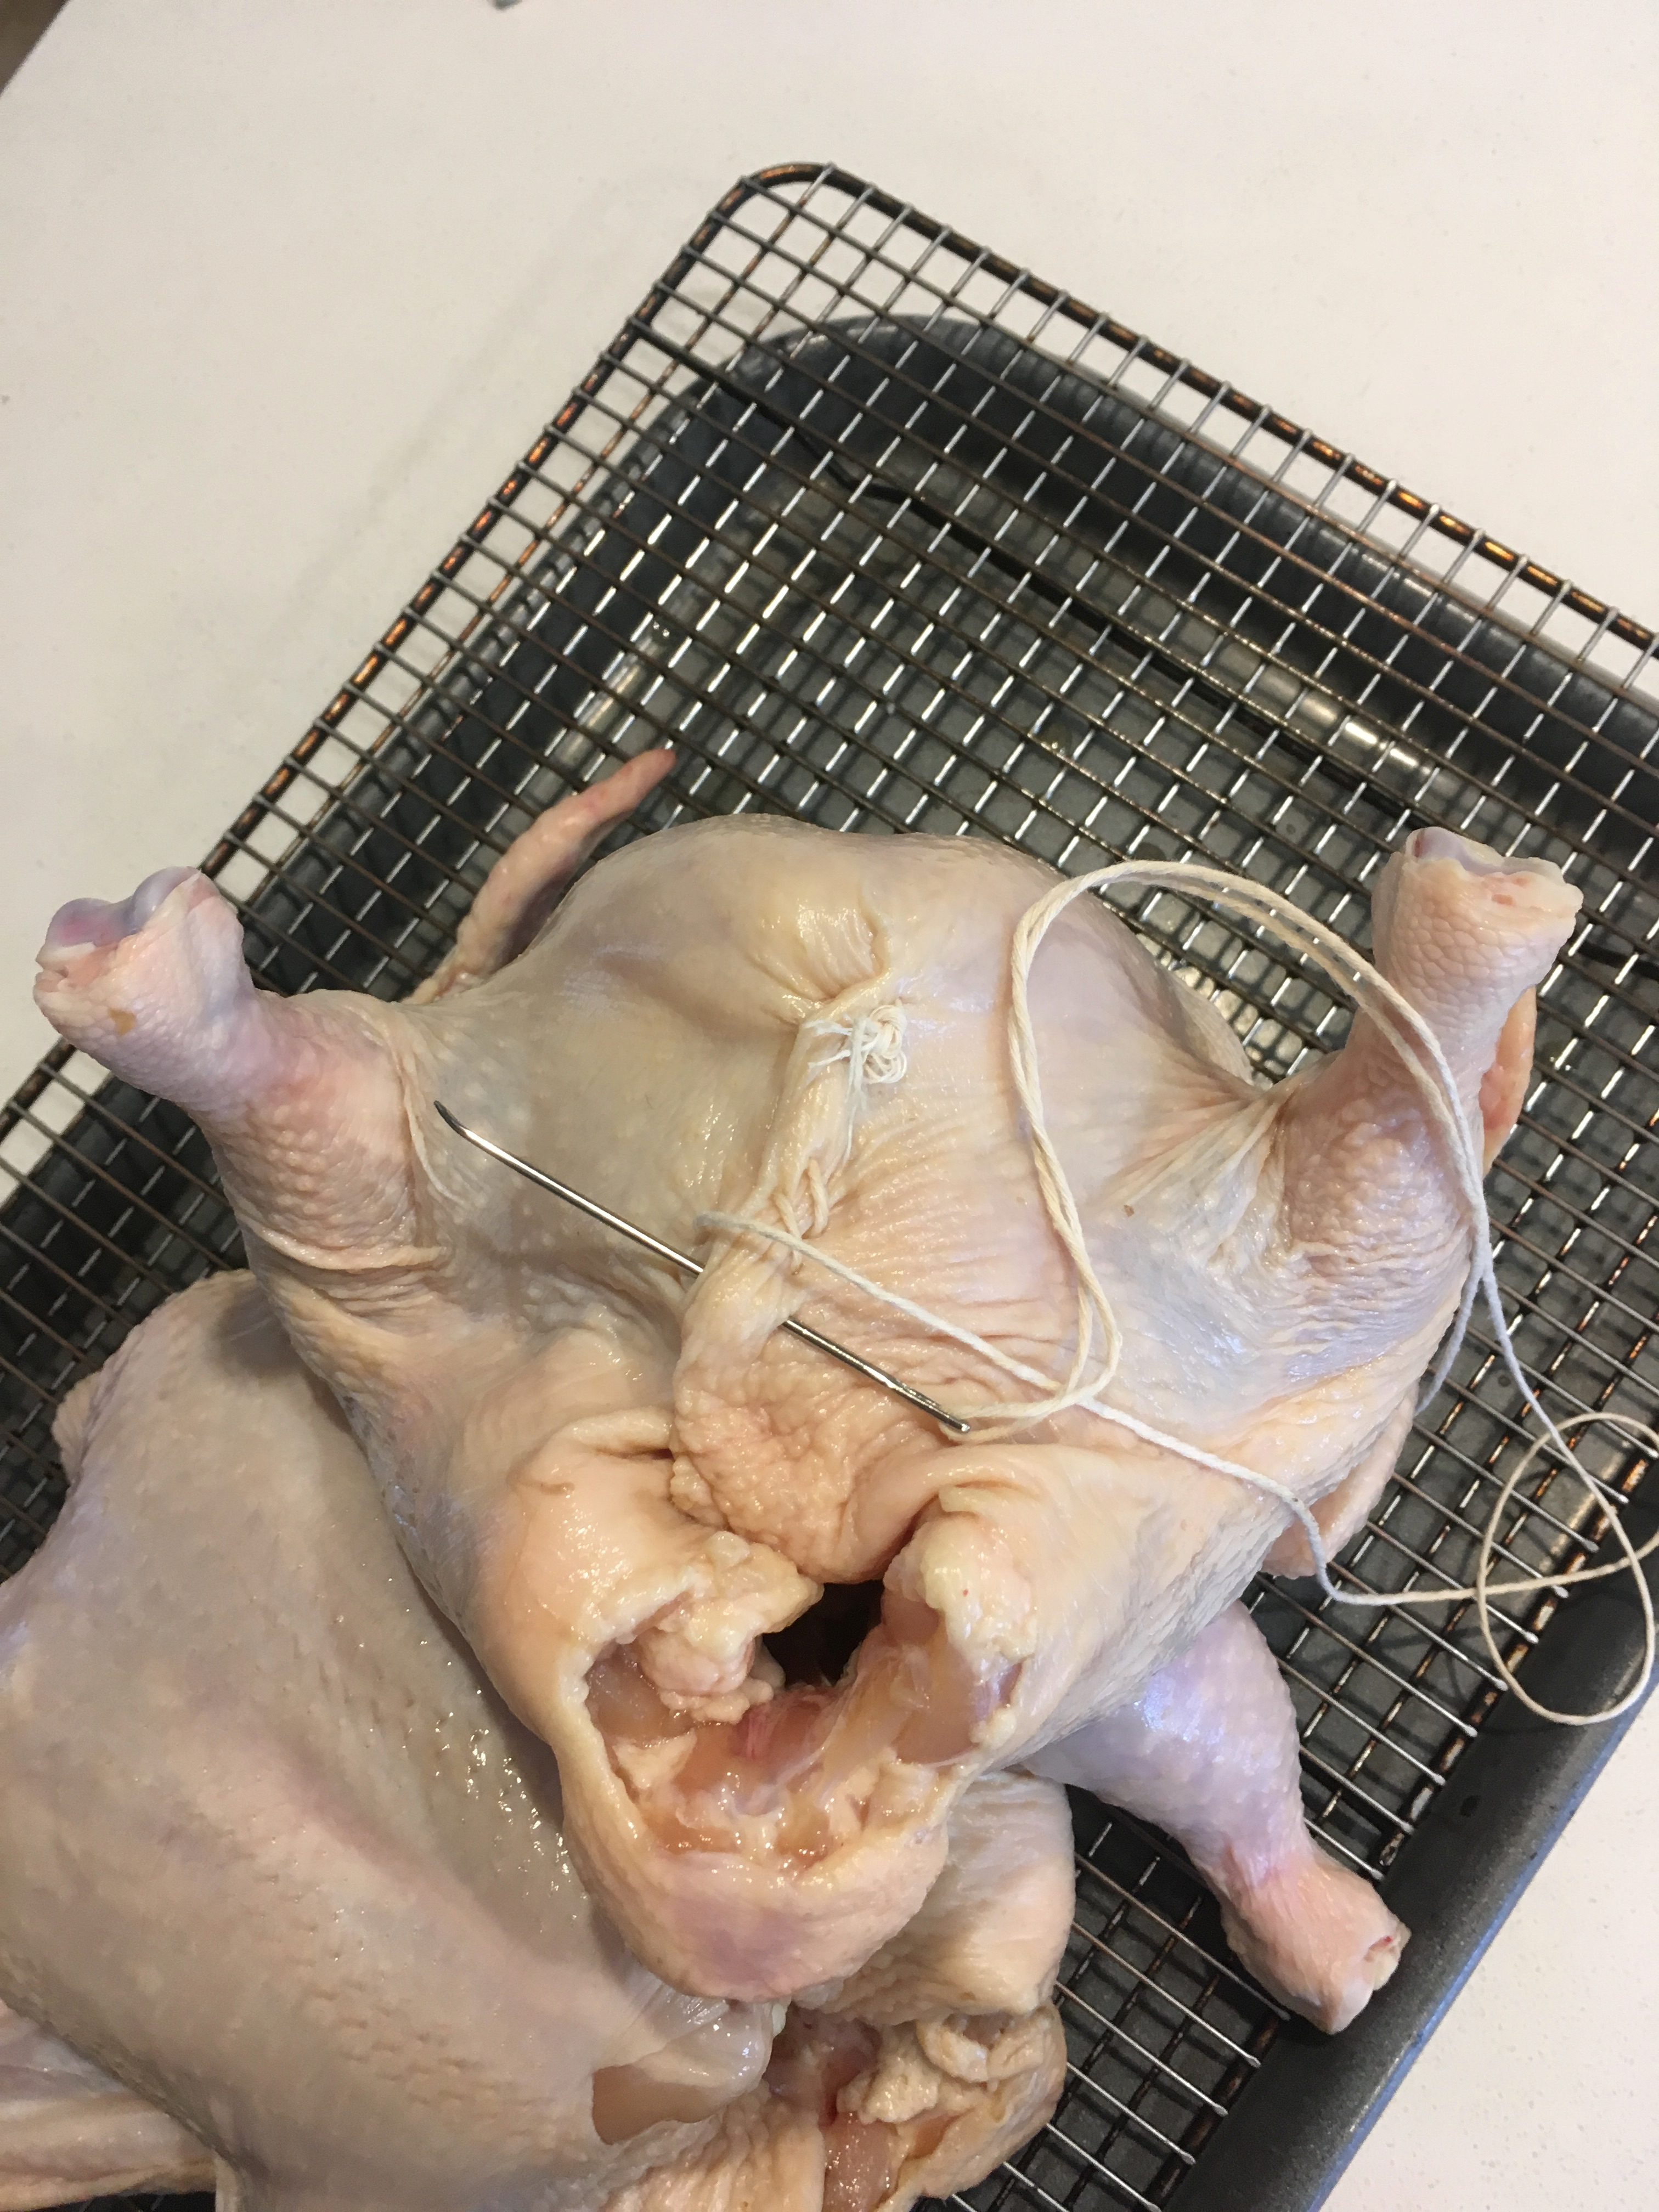
\includegraphics[width=0.25\textwidth]{\imageDir/\fileName/IMG_3216.jpg} \\
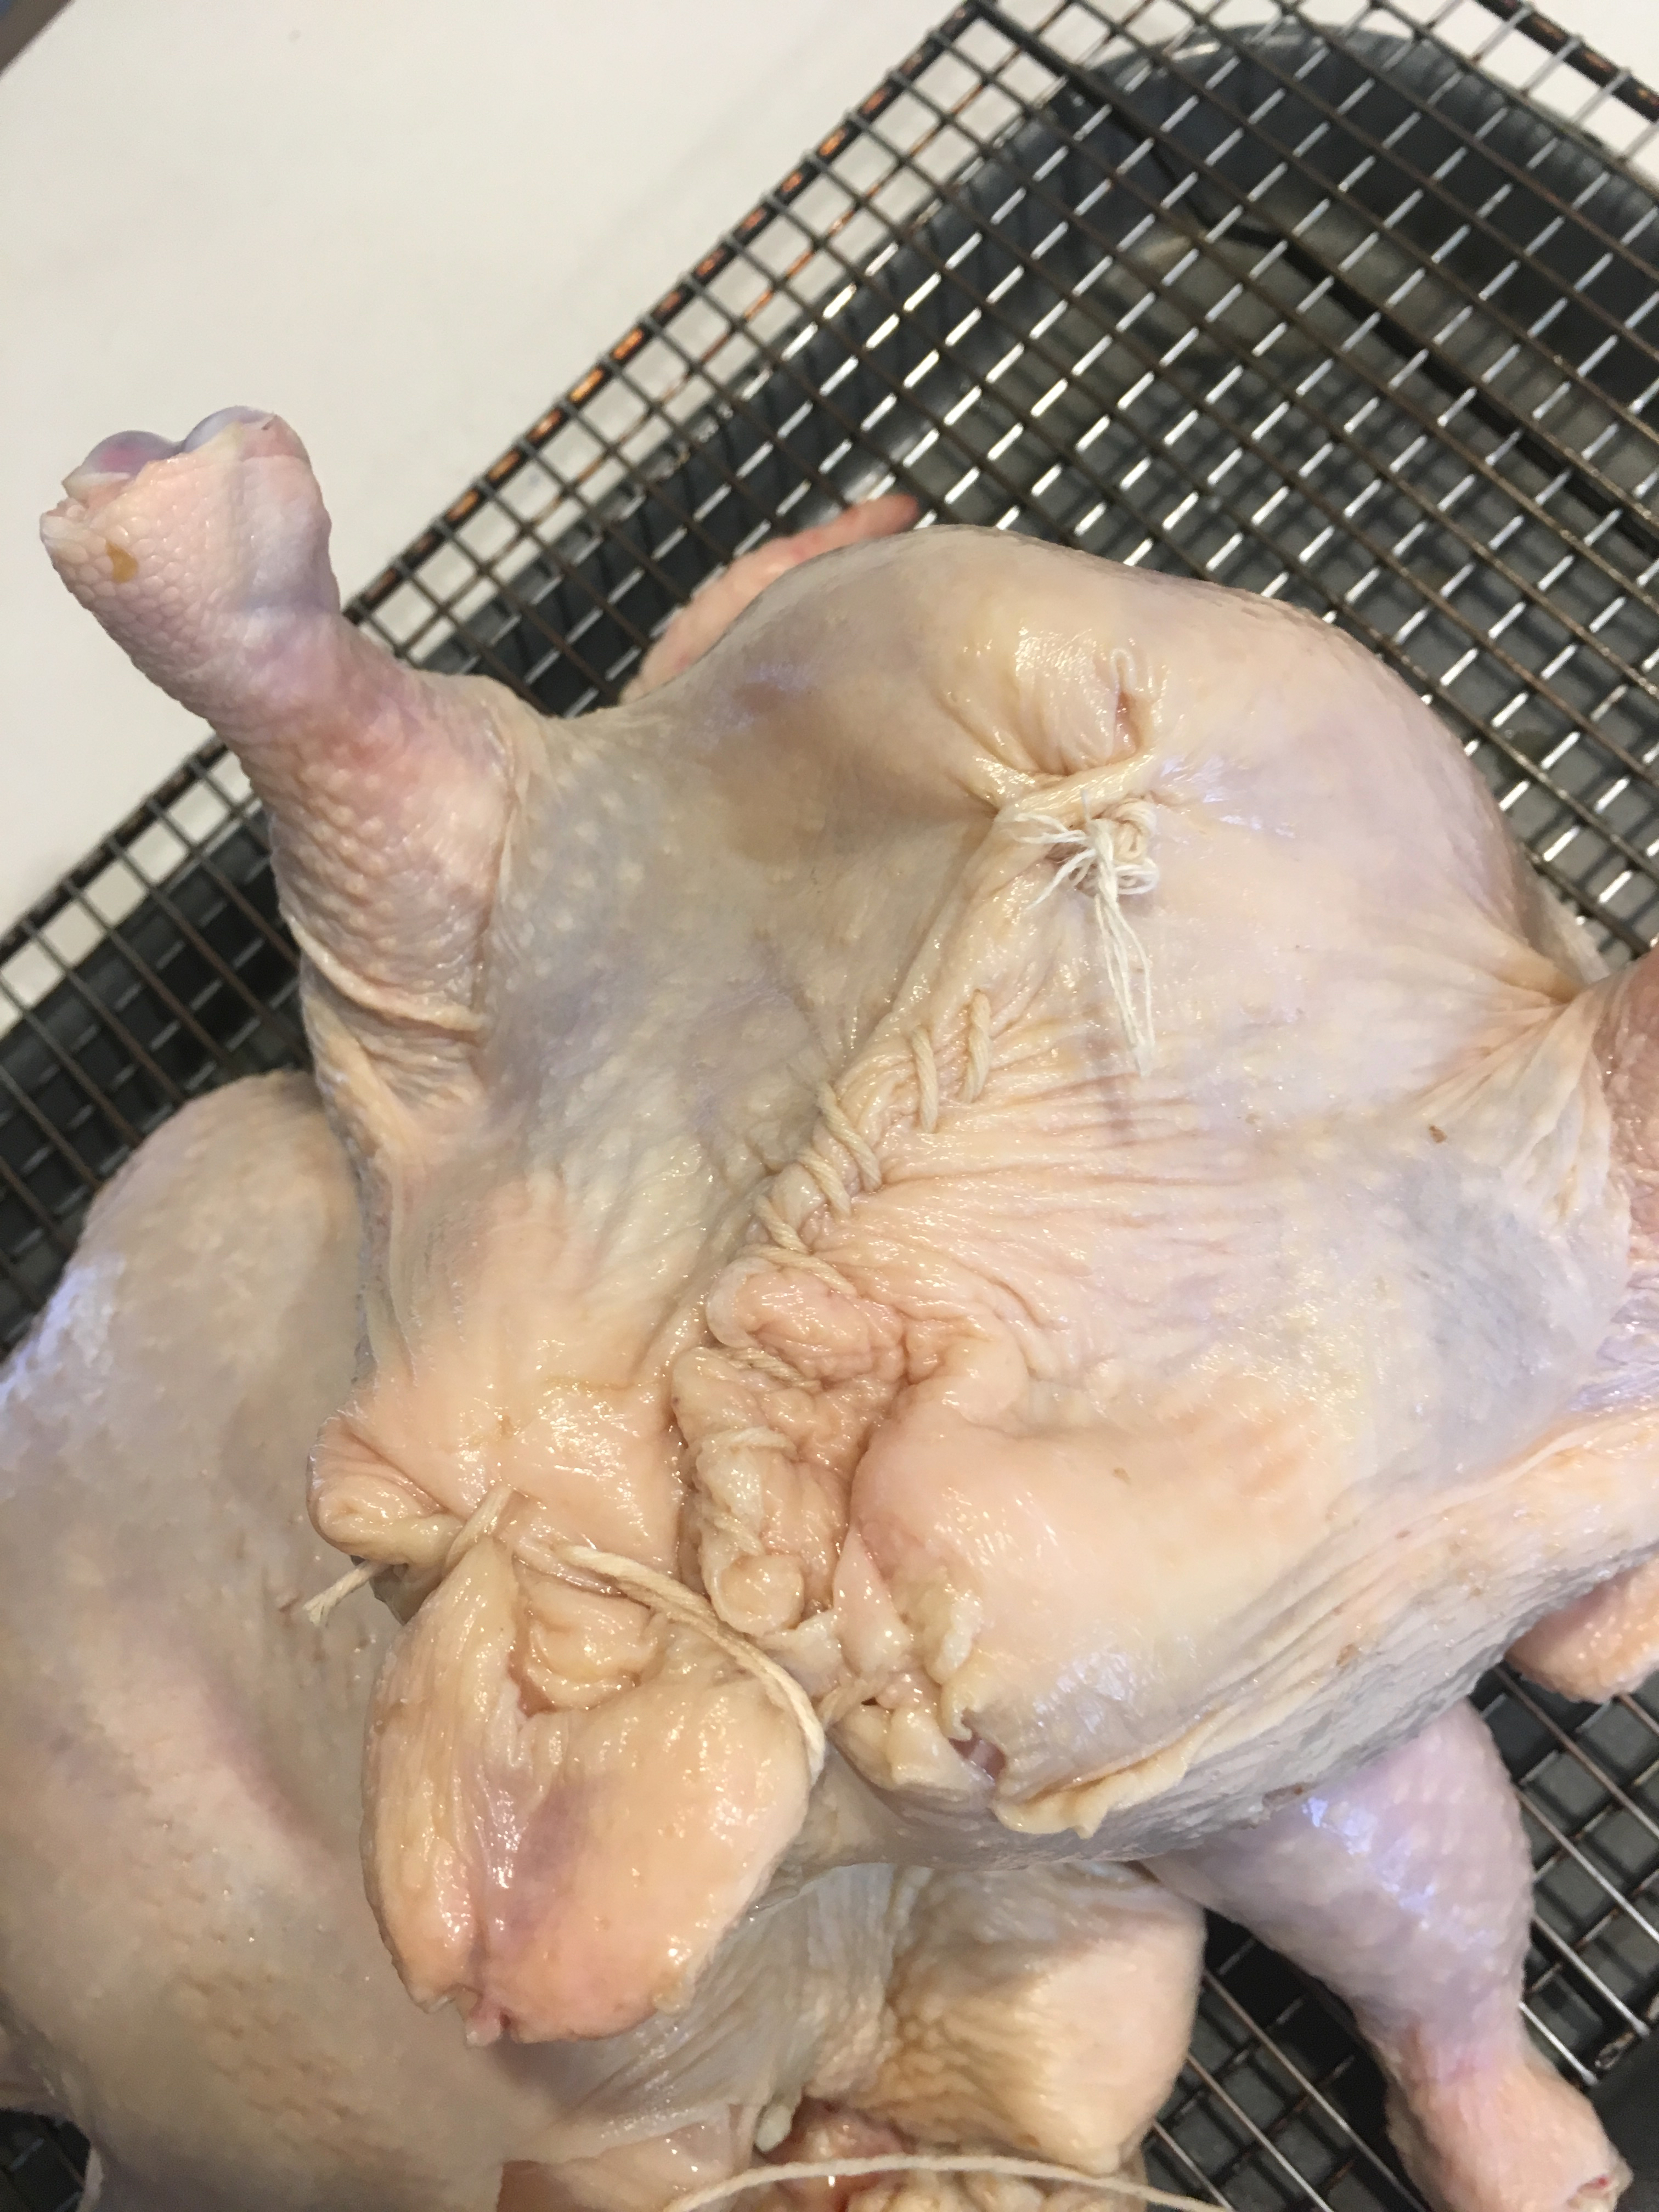
\includegraphics[width=0.25\textwidth]{\imageDir/\fileName/IMG_3217.jpg} &
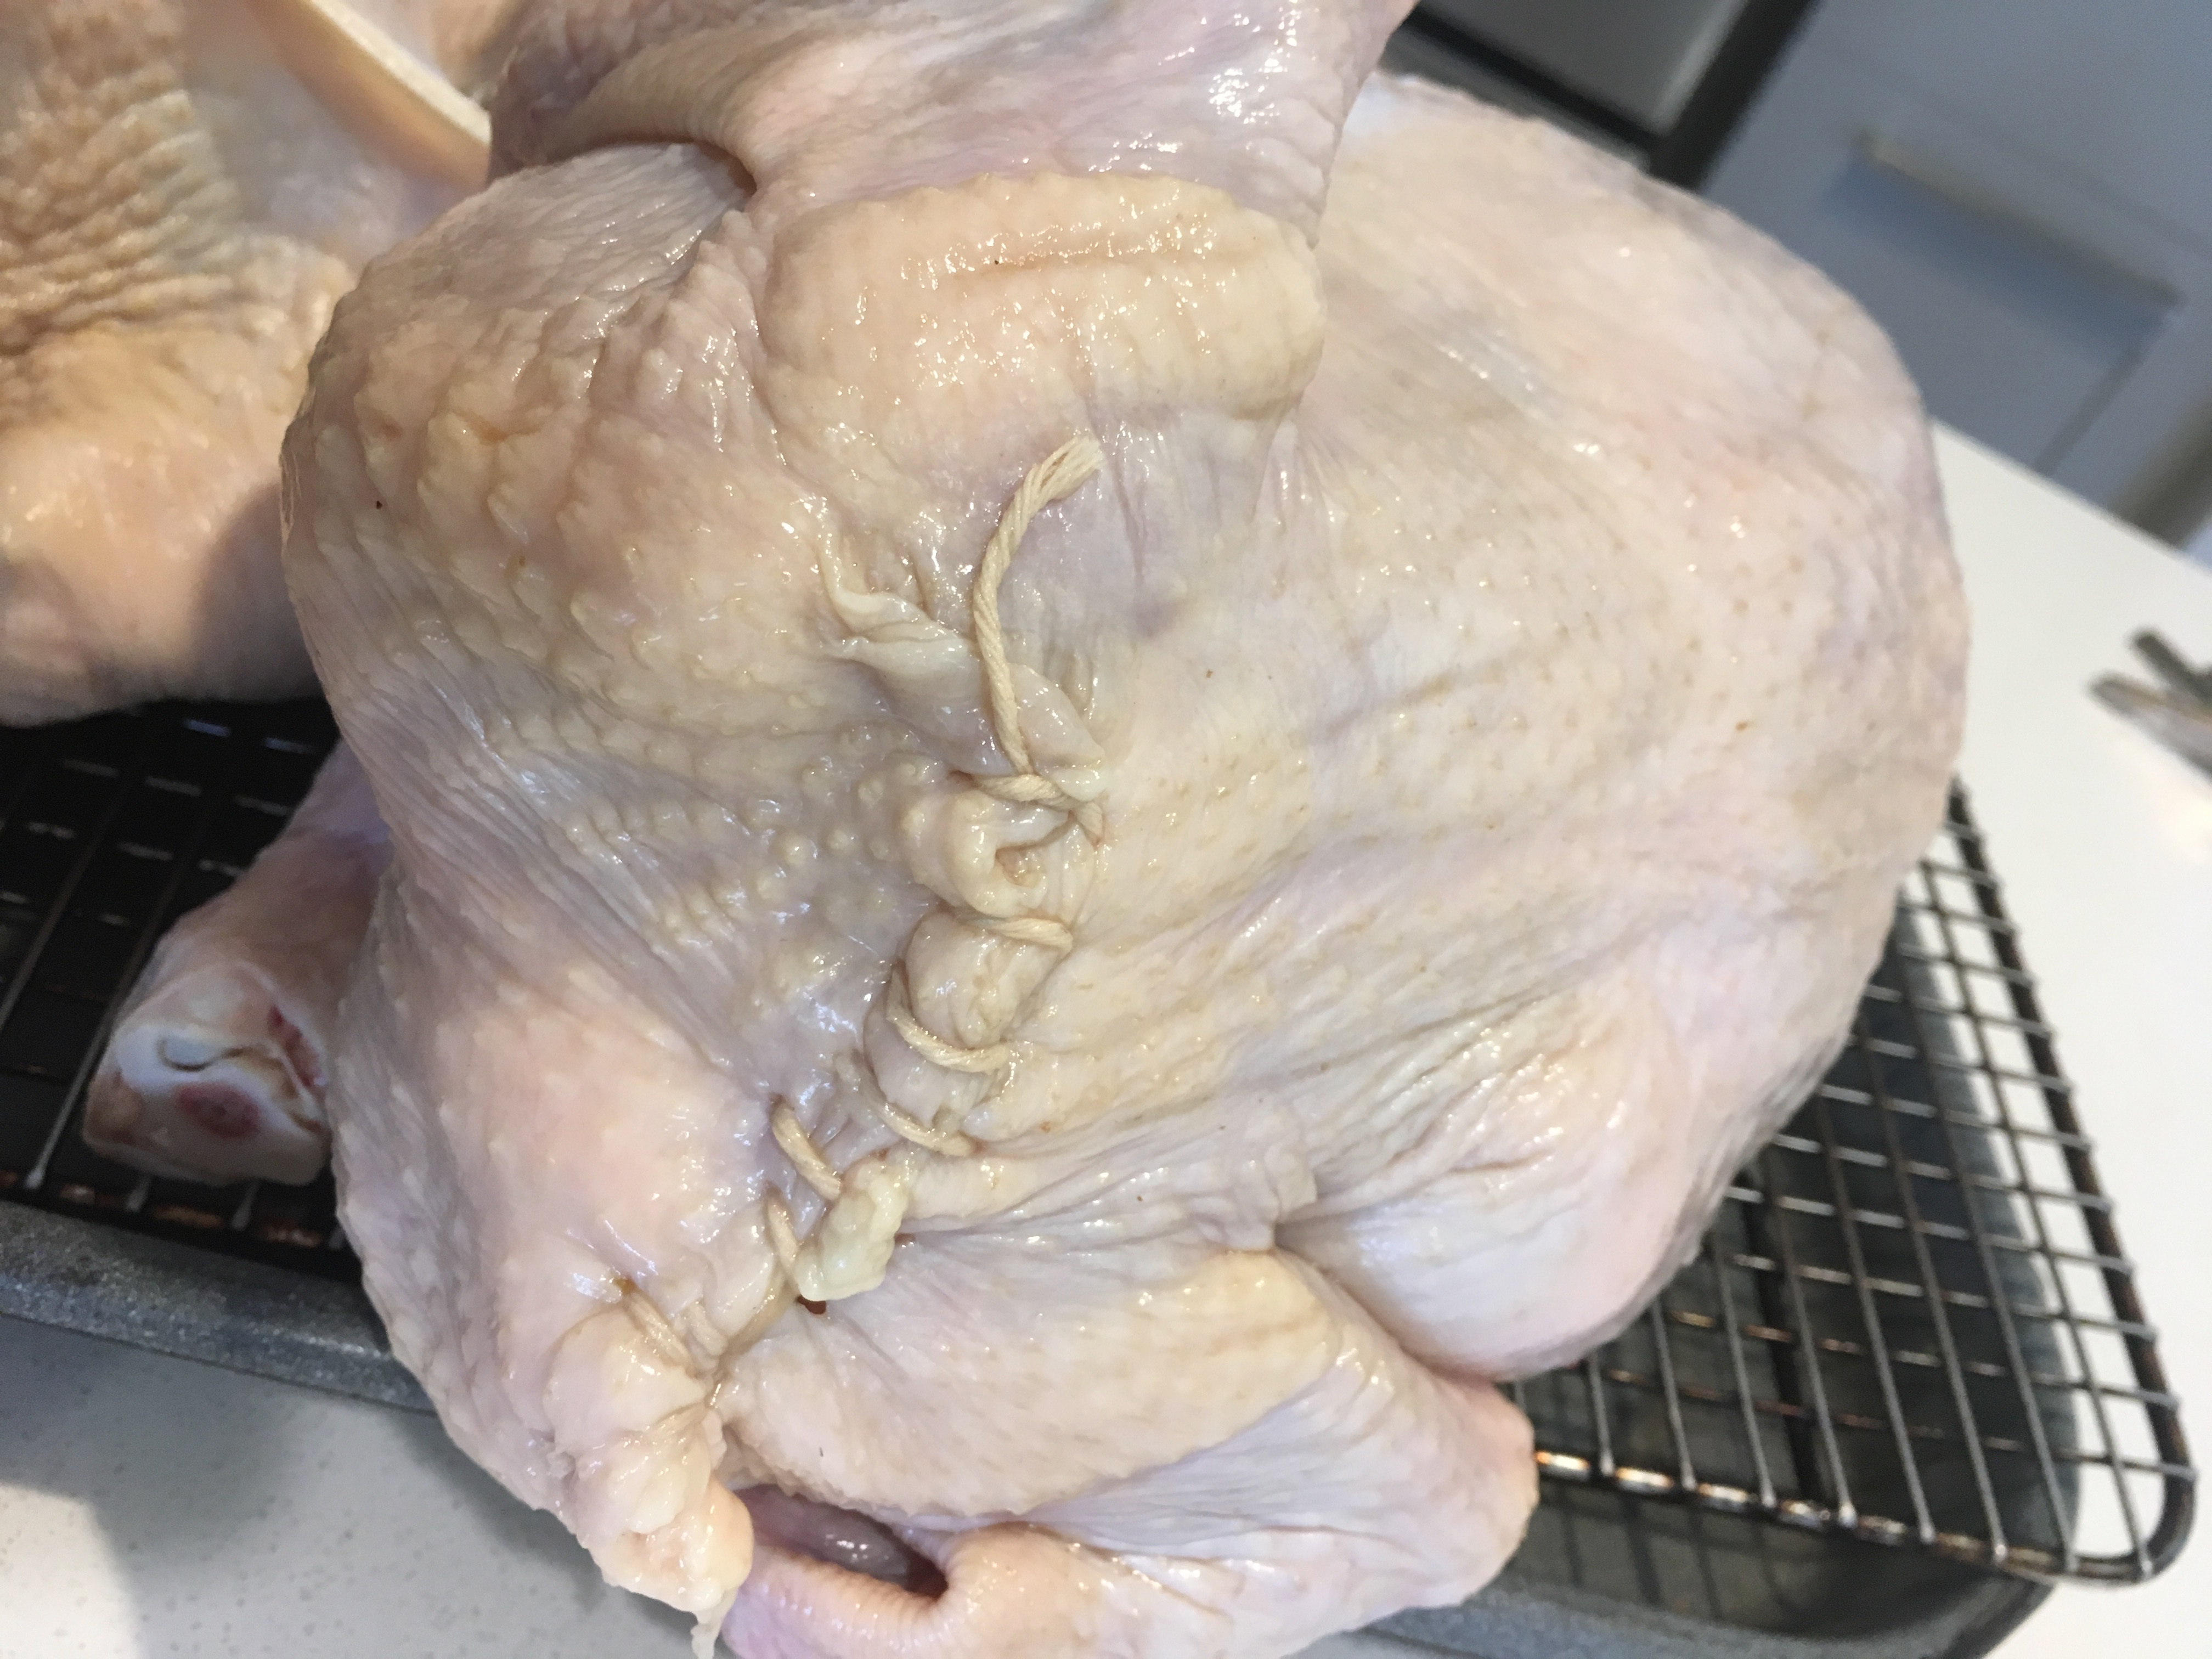
\includegraphics[width=0.25\textwidth]{\imageDir/\fileName/IMG_3218.jpg} &
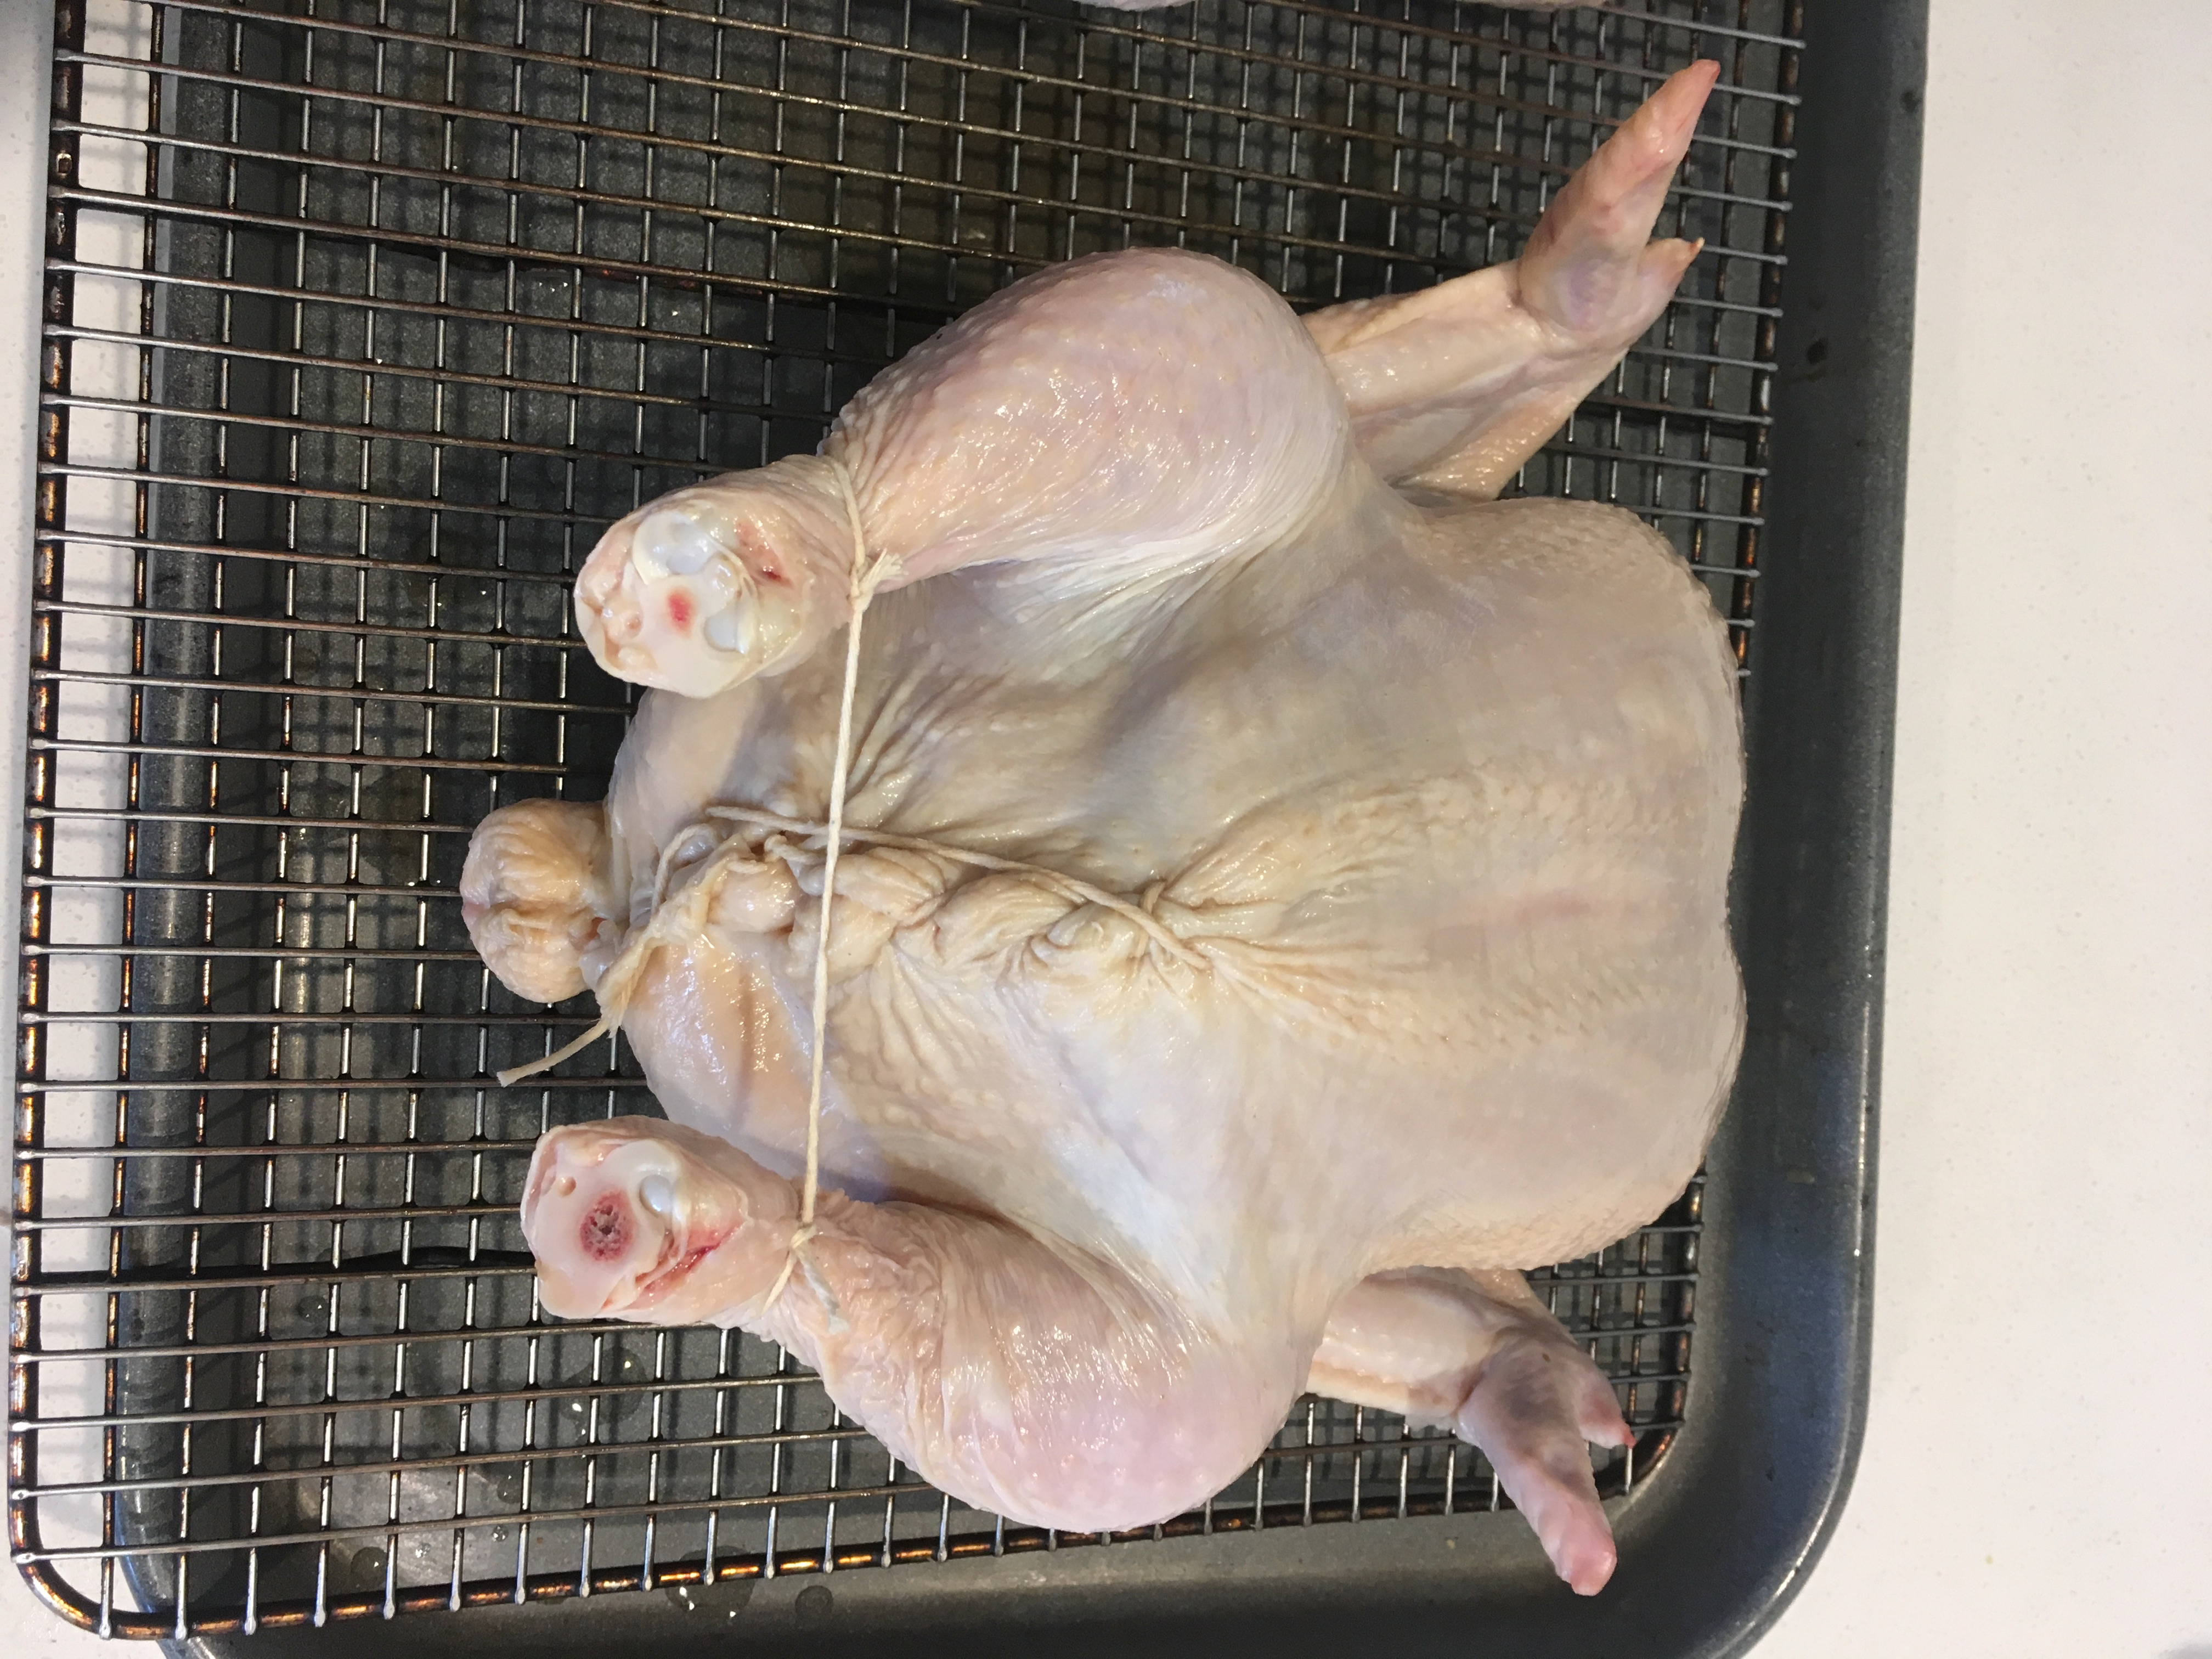
\includegraphics[width=0.25\textwidth]{\imageDir/\fileName/IMG_3219.jpg} \\
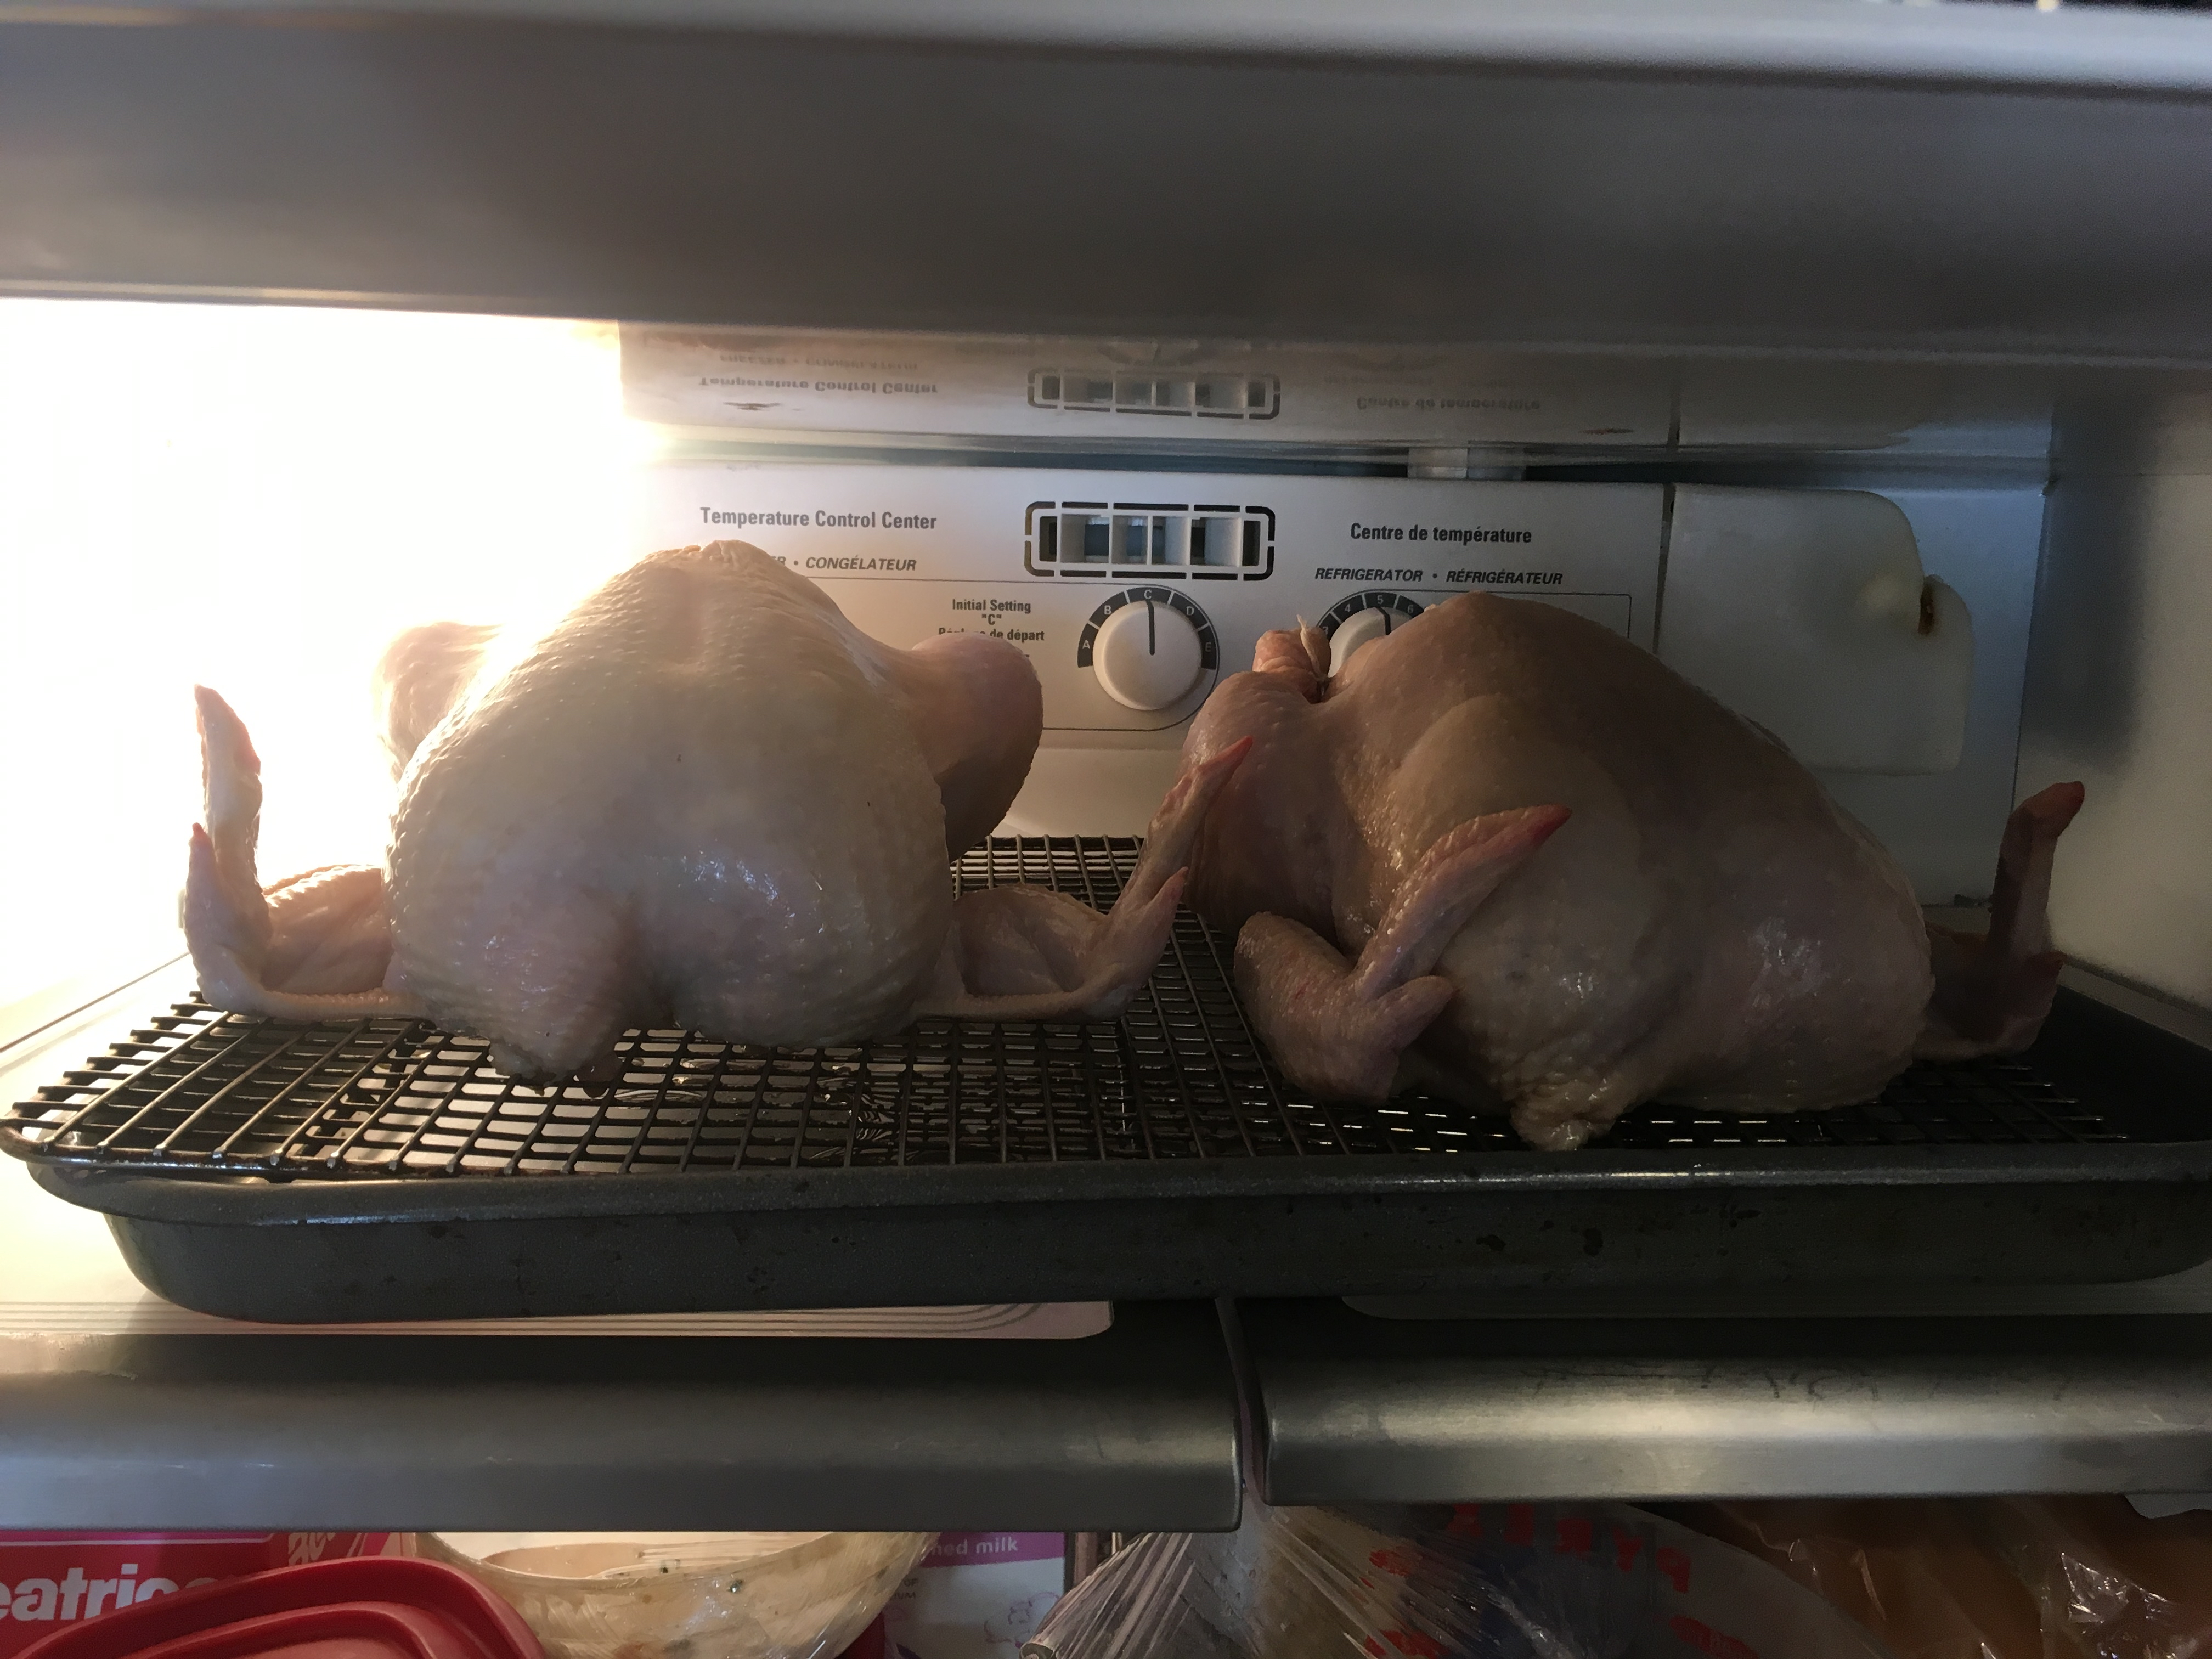
\includegraphics[width=0.25\textwidth]{\imageDir/\fileName/IMG_3220.jpg} &
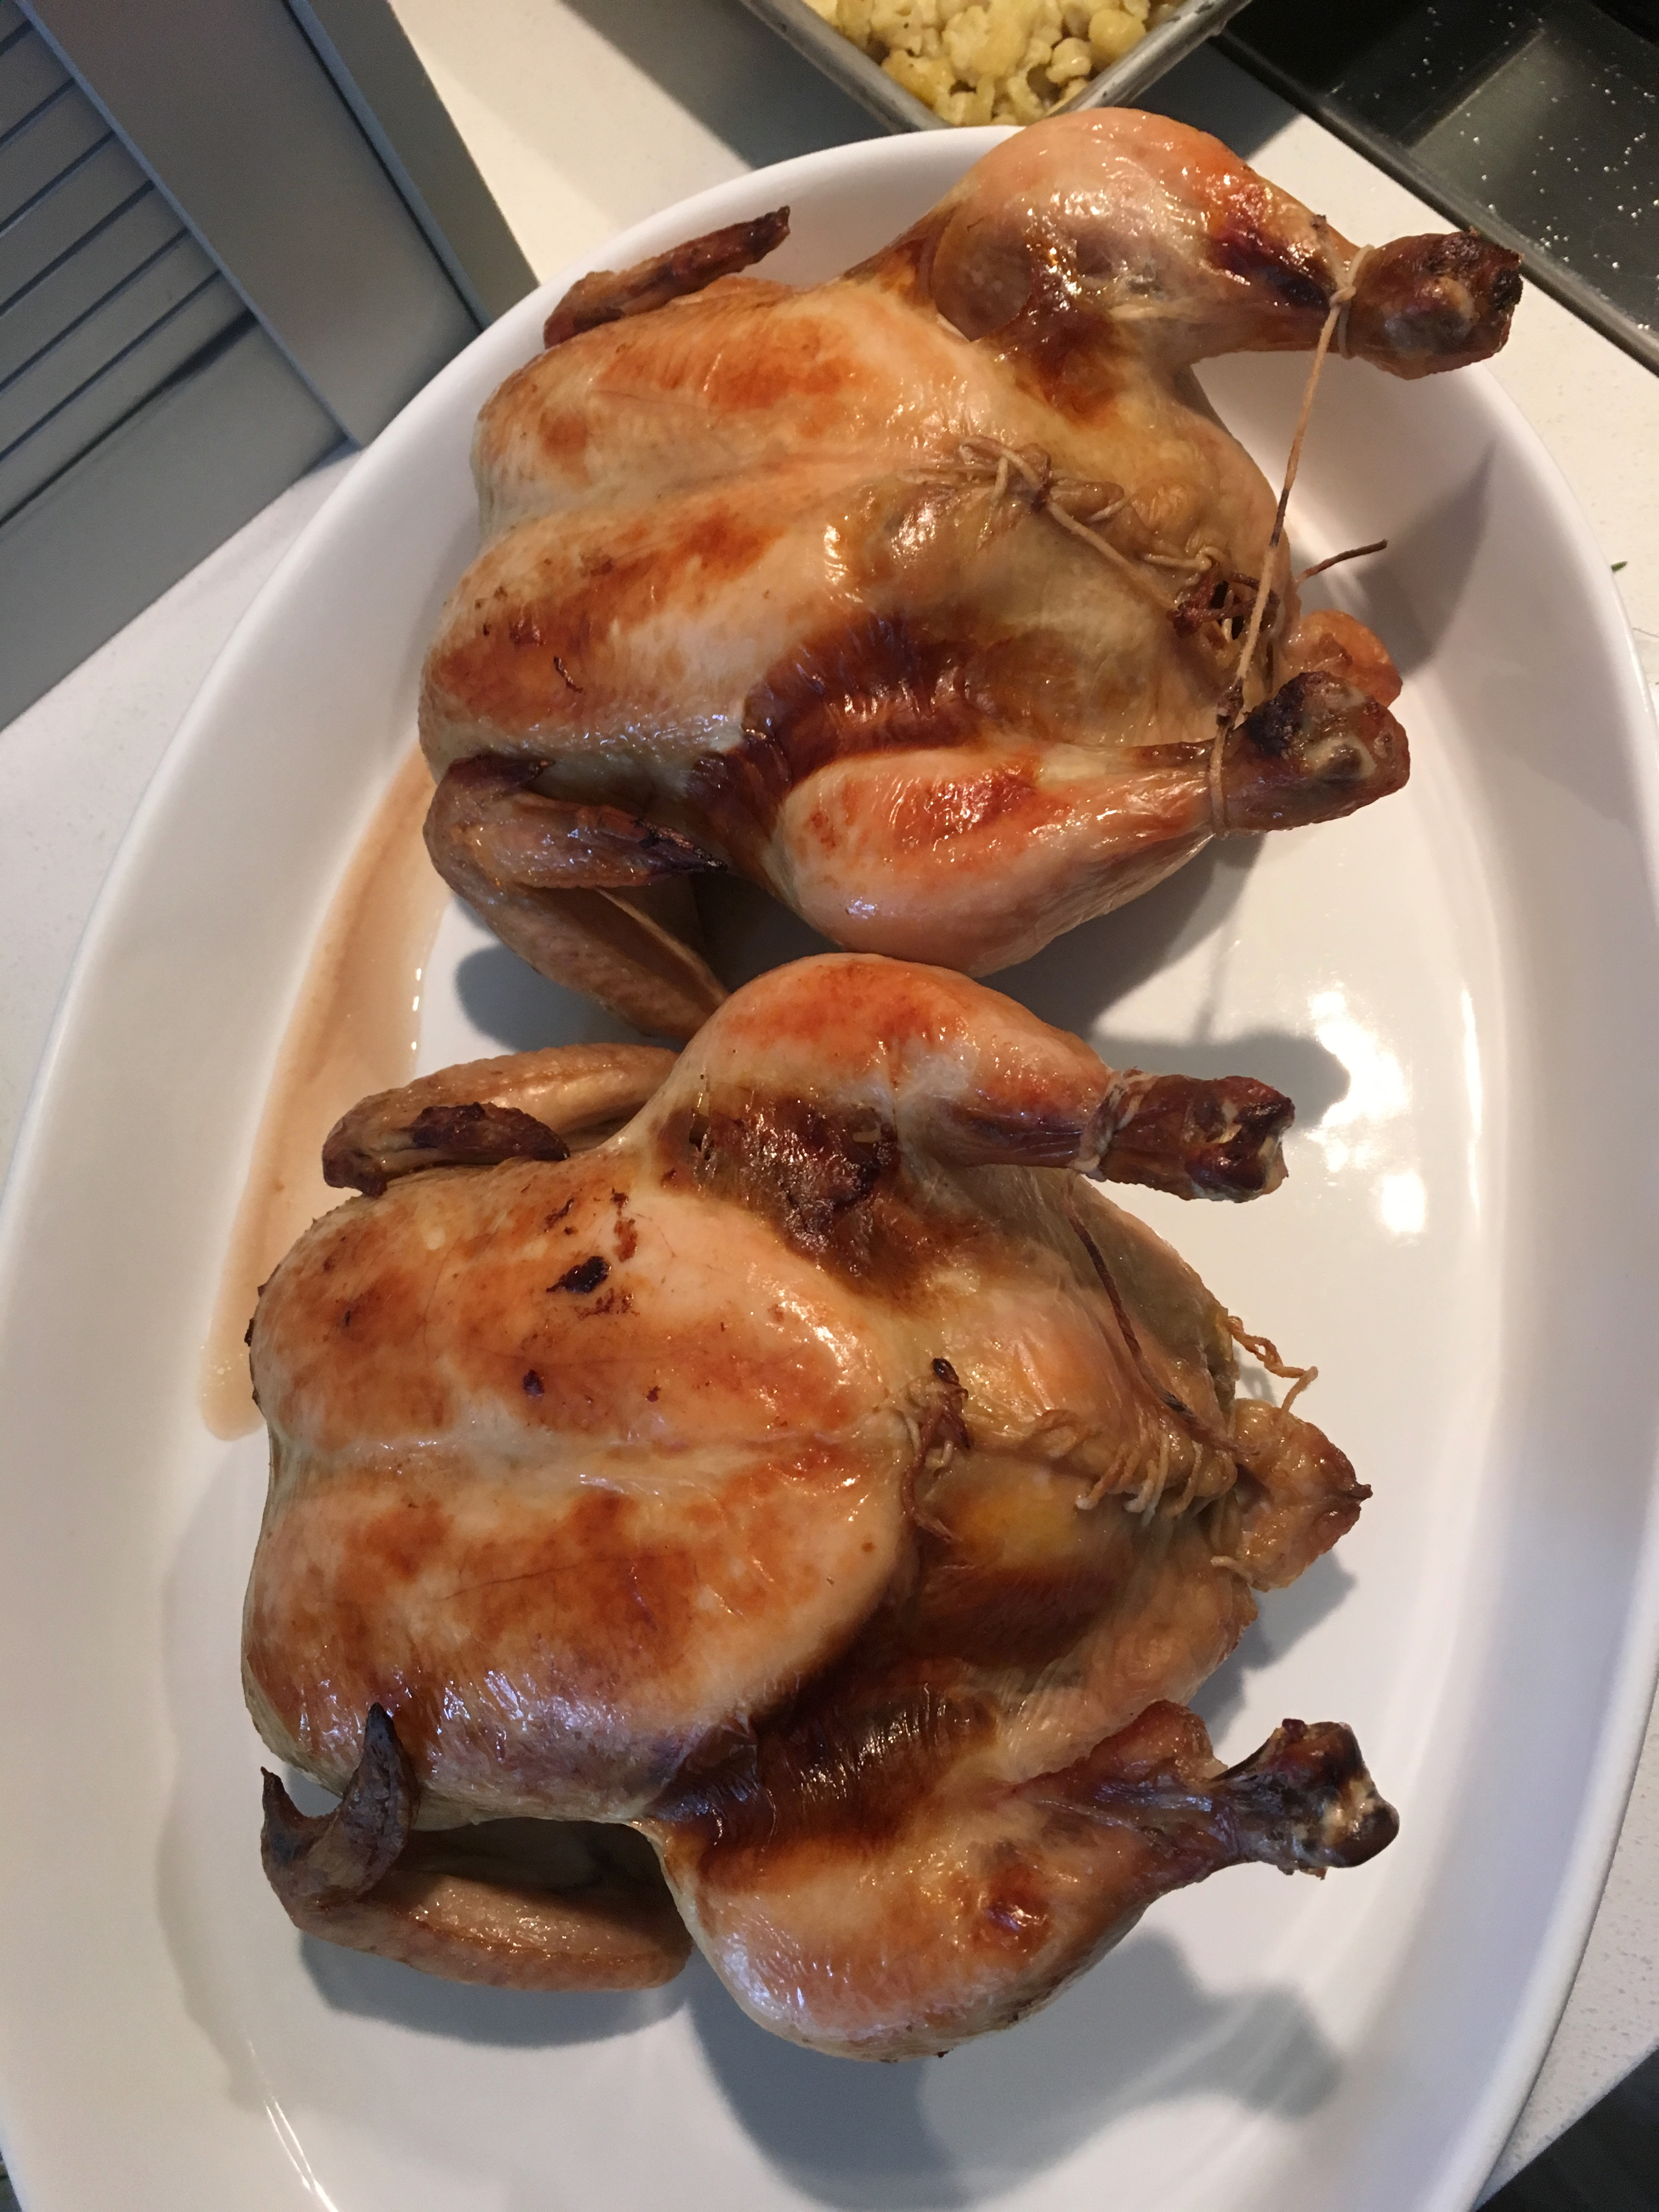
\includegraphics[width=0.25\textwidth]{\imageDir/\fileName/IMG_3228.jpg} \\
\end{tabular}
\end{table}


\end{document}
